\documentclass{article}

%%%%%%%%%%%%%%% LIBRERIAS %%%%%%%%%%%%%%%%%%%%%
\usepackage[thinc]{esdiff}
\usepackage{amsmath}
\usepackage{caption}
\usepackage{physics}
\usepackage{titlesec}
\usepackage{titletoc}
\usepackage{graphicx}
\usepackage[spanish,es-tabla]{babel} % 'es-tabla' cambia Cuadro→Tabla
\usepackage{hyperref}                % cargar después de babel
\usepackage{float}
\usepackage{circuitikz}
\usepackage[left=1.6cm,right=1.6cm,top=1.8cm,bottom=1.8cm]{geometry}
\usepackage{subfiles} 
\usepackage{subcaption}
\usepackage{pgfplots}
\pgfplotsset{compat=1.18}
\usepackage{booktabs} % Para tablas con tematica de paper cientifico
\usepackage{siunitx}  % Para alinear números en las tablas d:

%%%%%%%%%%%%%%%%%%% VARIABLES %%%%%%%%%%%%%%%%%%%%
\newcommand{\Facultad}{Instituto Tecnológico \\de\\ Buenos Aires} %constantes
\newcommand{\TPn}{Trabajo Práctico N° 1}
\newcommand{\TPtema}{Caracterización del amplificador operacional: medición de $A_{OL}$
 y análisis de sus limitaciones físicas}
\renewcommand{\thesection}{\arabic{section}}          % 2
\renewcommand{\thesubsection}{\quad \alph{subsection}}   % a
\renewcommand{\thesubsubsection}{\quad \thesubsection.~\roman{subsubsection}} % a. i
\graphicspath{{imagenes/}} %para que acceda a las fotos en la carpeta directamente


%%%%%%%%%%%%%%%%%% FORMATO TÍTULO Y NUMERACIÓN %%%%%%%%%%%%%%%%%%%
% Numeración de secciones
\renewcommand{\thesection}{\arabic{section}.}          
\renewcommand{\thesubsection}{\thesection\arabic{subsection}}       
\renewcommand{\thesubsubsection}{$\alph{subsubsection})$}

% Numerar hasta subsubsecciones
\setcounter{secnumdepth}{3}

% Formato de títulos
\titleformat{\section}{\Large\bfseries}{\thesection}{1em}{}
\titleformat{\subsection}{\large\bfseries}{\thesubsection}{0.5em}{}
\titleformat{\subsubsection}{\large\bfseries}{\thesubsubsection}{0.5em}{}



%%%%%%%%%%%%%%%%%%% ARCHIVO %%%%%%%%%%%%%%%%%%%%%%%%
\begin{document}

%%%CARATULA%%%
\begin{titlepage} %creo portada

        \begin{flushleft}
            \centering
            
\includegraphics[width=0.3\textwidth]{imagenes/Logo_ITBA.png}
        \end{flushleft}

        \centering
            
        {\scshape\LARGE \Facultad \par} %\par sirve para indicar un final de parrafo
        \vspace{1cm}                    %esto hace un espacio entre lineas de 1cm


        {\huge\bfseries \TPn \par}
        \vspace{1.5cm}
        {\Large Teoría de Circuitos 2\\ 25.14 \par}
        \vspace{0.5cm}
        {\Large \TPtema \par}
        \vfill                      %sirve para rellenar el espacio y quede simétrico.
        {\Large \bfseries Profesores: \par}
        \vspace{0.5cm}
         {\large  Daniel Jacoby \par Javier Petrucci \par Juan Sbruzzi \par Candela Gioia \par}
        \vspace{2cm}
        {\large Alumno: Juan Ignacio Caorsi \hfill Legajo: 65532  \par}
        \vfill
        {\large \today\par}
        \vfill

\end{titlepage}


\begingroup
  % Redefinimos temporalmente la sección que genera el título del índice
  \makeatletter
  \renewcommand{\section}{\@startsection{section}{1}{\z@}%
    {-3.5ex \@plus -1ex \@minus -.2ex}%
    {2.3ex \@plus .2ex}%
    {\Huge\bfseries}} % <--- Aquí defines el nuevo tamaño (ej. \Huge, \LARGE)
  \makeatother

  \tableofcontents
\endgroup

\newpage

%%%%%%%%%%%%%%%%%%% CUERPO DEL INFORME %%%%%%%%%%%%%%%%%%%%%%%%

\section{Introducción}
En este trabajo, se estudió diferentes configuraciones de circuitos haciendo uso de diferentes Amplificadores
 Operacionales. Se buscó explicar las discrepancias entre la realidad y las simulaciones como también los fenónemos
  específicos de cada dispositivo. A su vez, se integró una sección que trata acerca de la forma de medir la ganancia
   a lazo abierto de los Op. Amp. con un circuito especial conocido como Servo Loop.
Aclaración: este trabajo buscaba estudiar el dispositivo TL082, pero dado que no fue posible utilizar uno en condiciones,
 se optó por realizar el análisis general para el TL072 y el modelo Spice del TL082, muy similar al anterior. Luego,
  para la obtención de la ganancia del dispositivo, se utilizó el TL082.

\section{Amplificador Operacional TL072: ejemplo de funcionamiento en configuración inversora}
    Se tiene el circuito de la figura \ref{fig:Ej1}, que consiste en un amplificador operacional TL072 configurado 
    como amplificador inversor. La ganancia de este circuito, considerado ideal, está determinada por la expresión
     $\frac{V_{o}}{V_{in}} = -\frac{R_1}{R_2} = -2,2$, si se considera a las resistencias de $R1=3,3k\Omega$ y $R2=1,5k\Omega$. 
     La señal de Vin es una senoidal de frecuencia 1kHz y amplitud 1V. 
    Una vez medida experimentalmente la salida del circuito se compara con la simulación realizada en el software LTSpice en la figura \ref{fig:Ej11}.



\begin{figure}[htbp]
    \centering
    % Primera imagen
    \begin{minipage}[t]{0.55\textwidth}
        \centering
        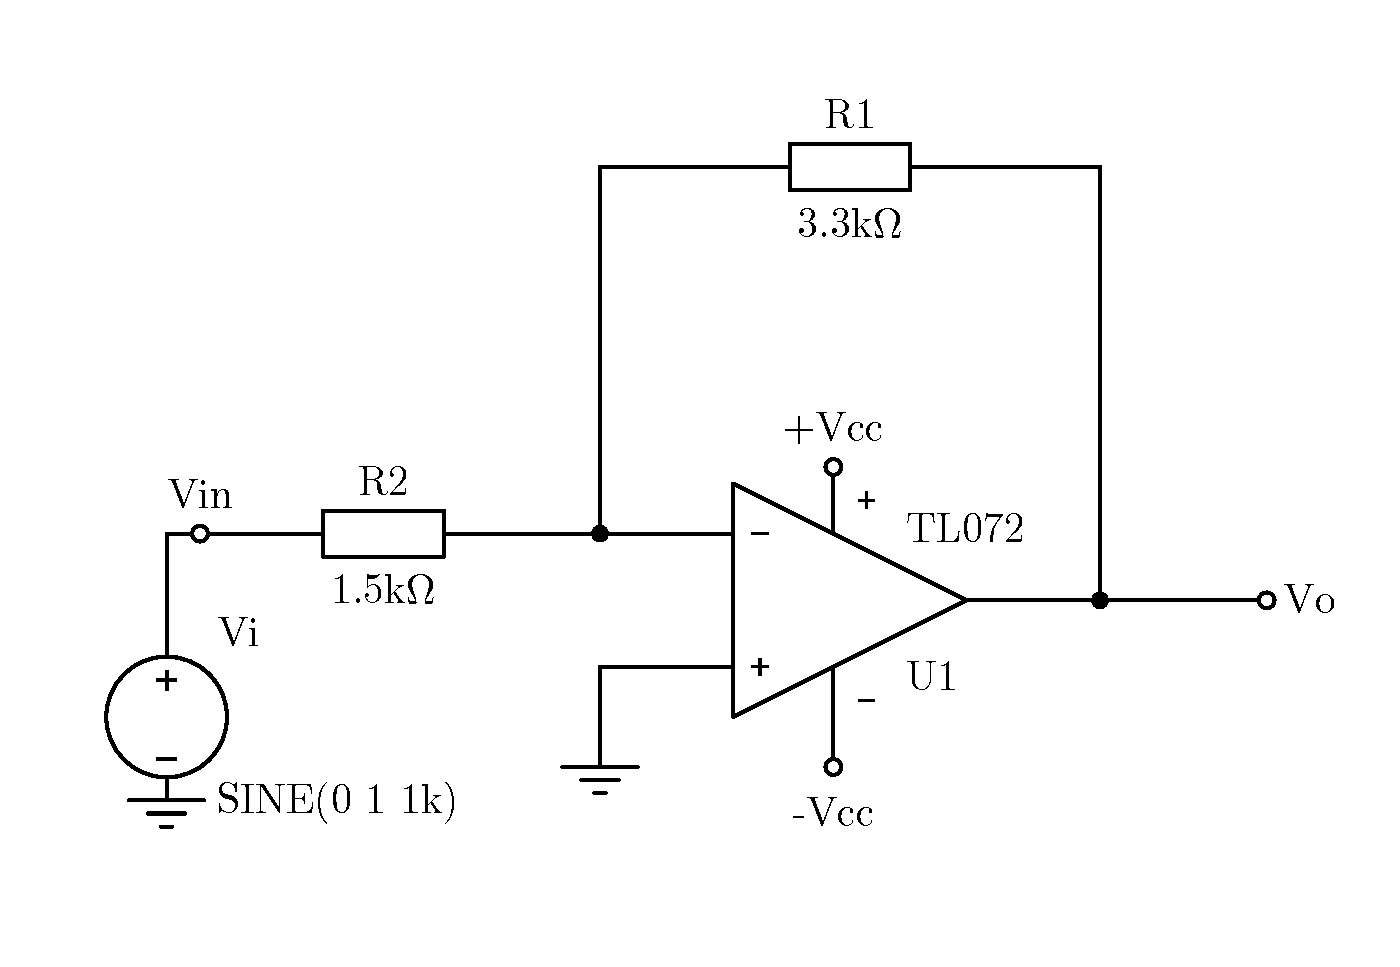
\includegraphics[width=\textwidth]{Ej1.pdf} 
        \caption{Circuito analizado, configuración inversora.
         Con Vcc-=-15V, Vcc+=+15V.}
         \label{fig:Ej1}
    \end{minipage}
    \hfill % Espacio horizontal automático entre ambas imágenes
    % Segunda imagen
    \begin{minipage}[t]{0.35\textwidth}
        \centering
        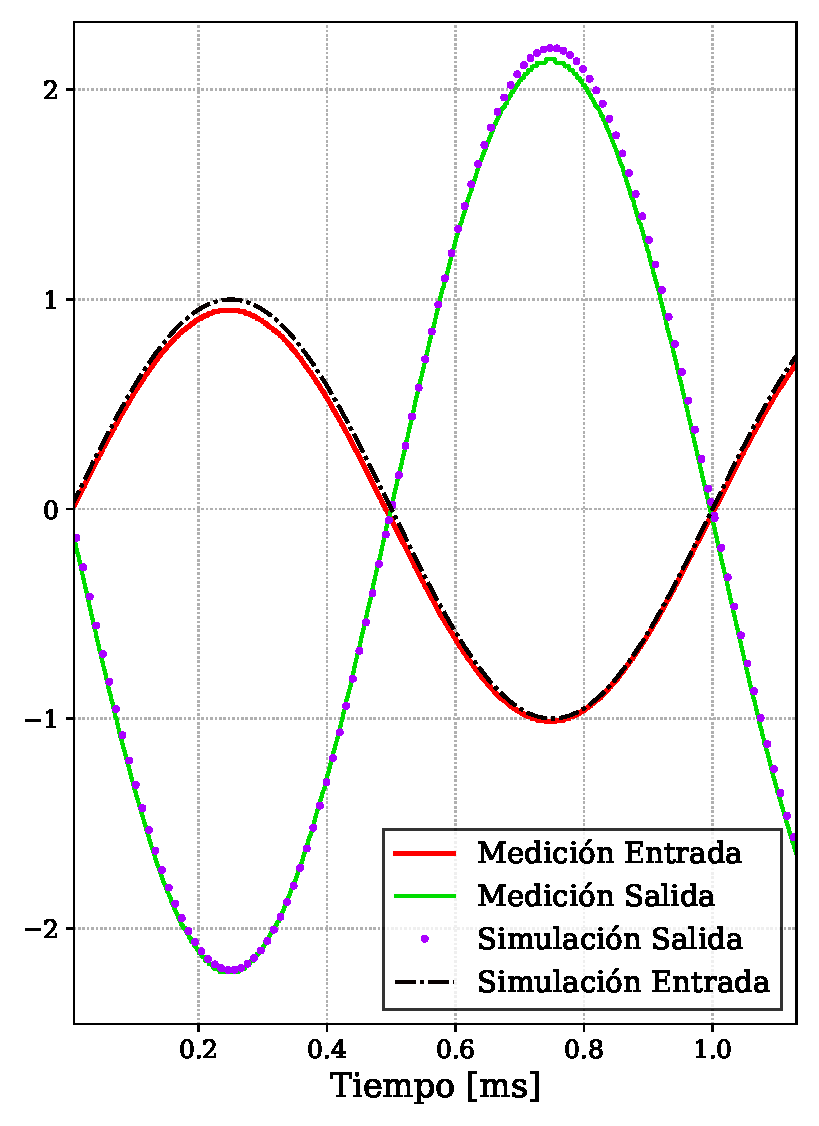
\includegraphics[width=\textwidth]{ej1a_teoprac.pdf} 
        \caption{Simulación y medición del circuito analizado, en configuración inversora. La línea punteada y la línea con segmentos-puntos son la salida y la entrada de la simulación respectivamente, mientras que las líneas continuas verde y roja son la salida y la entrada de la medición respectivamente en modo average.}
        \label{fig:Ej11}
    \end{minipage}
\end{figure}

Como la ganancia es de -2,2, es esperable que la amplitud de la señal de salida sea de 2,2V, y eso es justamente lo que se ve tanto en la simulación como en la medición,
excepto por una salvedad en el último caso: en la medición se puede ver el generador falla en alcanzar la tensión pico de 1V por 50mV, 
y lo mismo pasa con la salida al acercarse a 2,2V. Esto se puede deber a efectos parásitos de los elementos con los que se realizó el circuito por su no idealidad, al igual que la precisión de medición del osciloscopio (20mV).






Si se conectara la terminal no inversora a 1V, se vería que la salida es igual a la del circuito inversor anterior pero con un
offset de 3,2V. Esto se puede justificar teóricamente con la resolución del circuito por el método de superposición, 
considerando la suma de la señal de salida ya vista en la figura \ref{fig:Ej11} y la salida del circuito inversor ideal con la terminal 
no inversora conectada a 1V. Lo medido se puede ver en la figura \ref{fig:Ej111}, y la simulación es coherente con lo visto.

\begin{figure}[htbp]
    \centering
    % Ajusta el ancho con respecto al texto (ej. 80% del ancho del texto)
    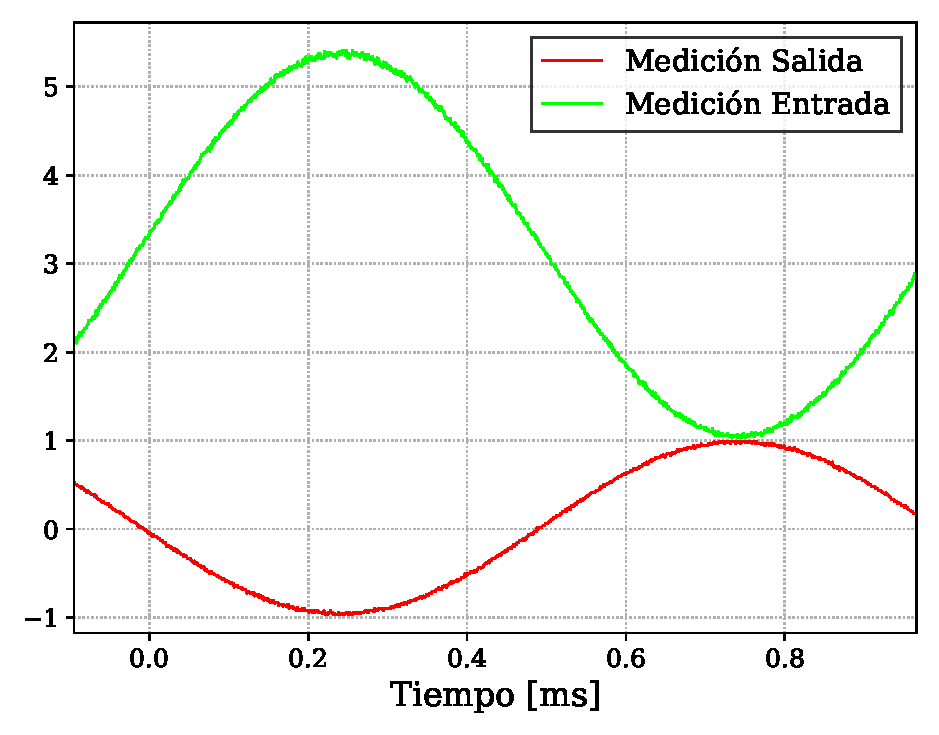
\includegraphics[width=0.5\textwidth]{ej1a_teoprac1V.pdf} 
    \caption{Medición del circuito inversor con la terminal no inversora a 1V. Los valores pico de la salida son 5,4V y 1V. Vin (curva roja), Vout (curva verde)}
    \label{fig:Ej111}
\end{figure}

\section{Análisis de funcionamiento y limitaciones de los Op. Amp. TL072 y LM741}
    En esta sección, se analizó un circuito como el de la figura \ref{fig:Ej2buffer} para cada uno de los casos 
    listados en la tabla \ref{tab:Ej2}. Se compararon los resultados obtenidos experimentalmente con los de la simulación realizada en el software LTSpice.

\begin{table}[H]
\centering
\begin{tabular}{|c|c|c|c|c|c|c|c|}
\hline
Caso & $+V_{cc}\ [\text{V}]$ & $-V_{cc}\ [\text{V}]$ & $V_{DC}\ [\text{V}]$ & $V_p\ [\text{V}]$ & $f_{in}\ [\text{Hz}]$ & $R_L\ [\Omega]$ & Integrado \\ \hline
A & 10 & -10 & 0 & 1 & 100 & $\infty$ & TL072 \\ \hline
B & 10 & -10 & 0 & 10 & 100 & $\infty$ & LM741 \\ \hline
C & 10 & -2 & 0 & 3 & 100 & $\infty$ & TL072 y LM741 \\ \hline
D & 4 & -4 & 3.5 & 1 & 100 & $\infty$ & TL072 \\ \hline
E & 10 & -10 & 0 & 5 & 100 & 100 & TL072 \\ \hline
F & 10 & -10 & 0 & 10 & 100 & 560 & LM741 \\ \hline
G & 10 & -10 & 0 & 8 & 800k & $\infty$ & TL072 \\ \hline
\end{tabular}
\caption{Casos de estudio.}
\label{tab:Ej2}
\end{table}



\subsection{Caso A}

\begin{table}[H]
\centering
\begin{tabular}{|c|c|c|c|c|c|c|c|}
\hline
Caso & $+V_{cc}\ [\text{V}]$ & $-V_{cc}\ [\text{V}]$ & $V_{DC}\ [\text{V}]$ &
 $V_p\ [\text{V}]$ & $f_{in}\ [\text{Hz}]$ & $R_L\ [\Omega]$ & Integrado \\ \hline
A & 10 & -10 & 0 & 1 & 100 & $\infty$ & TL072 \\ \hline
\end{tabular}
\end{table}

Se compara la salida medida con la simulada en la figura \ref{fig:Ej2a}. 
Se observa que la salida medida es muy similar a la simulada, se nota que la medición tuvo ruido pero nada remarcable. 
Se omite la comparación con la señal de entrada pues es muy similar a la salida como se esperaba.


\begin{figure}[htbp]
    \centering
    % Primera imagen
    \begin{minipage}[t]{0.35\textwidth}
        \centering
        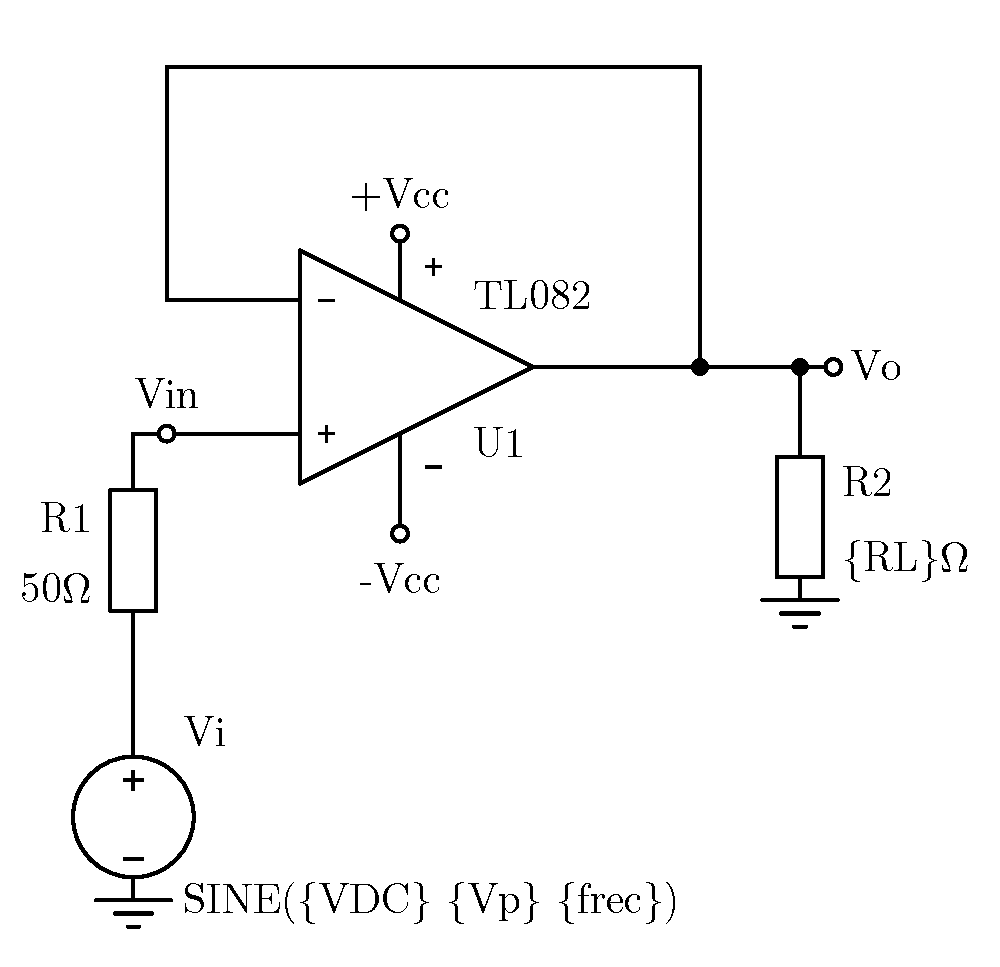
\includegraphics[width=\textwidth]{Ej2_buffer.pdf} 
        \caption{Circuito analizado, configuración buffer. Parámetros a considerar:
         señal de entrada: VDC (DC offset [V]), frec (frecuencia), Vp (amplitud de la senoidal), 
         RL (resistencia de carga), Vcc- y Vcc+ (tensión de alimentación), y el modelo del
          amplificador operacional. R1 representa la resistencia interna del generador de señales, notar que si se realiza el mismo análisis sin considerar dicha resistencia no hay diferencia apreciable, la corriente que la atraviesa es insignificante.}
        \label{fig:Ej2buffer}
    \end{minipage}
    \hfill % Espacio horizontal entre las dos imágenes
    % Segunda imagen
    \begin{minipage}[t]{0.6\textwidth}
        \centering
        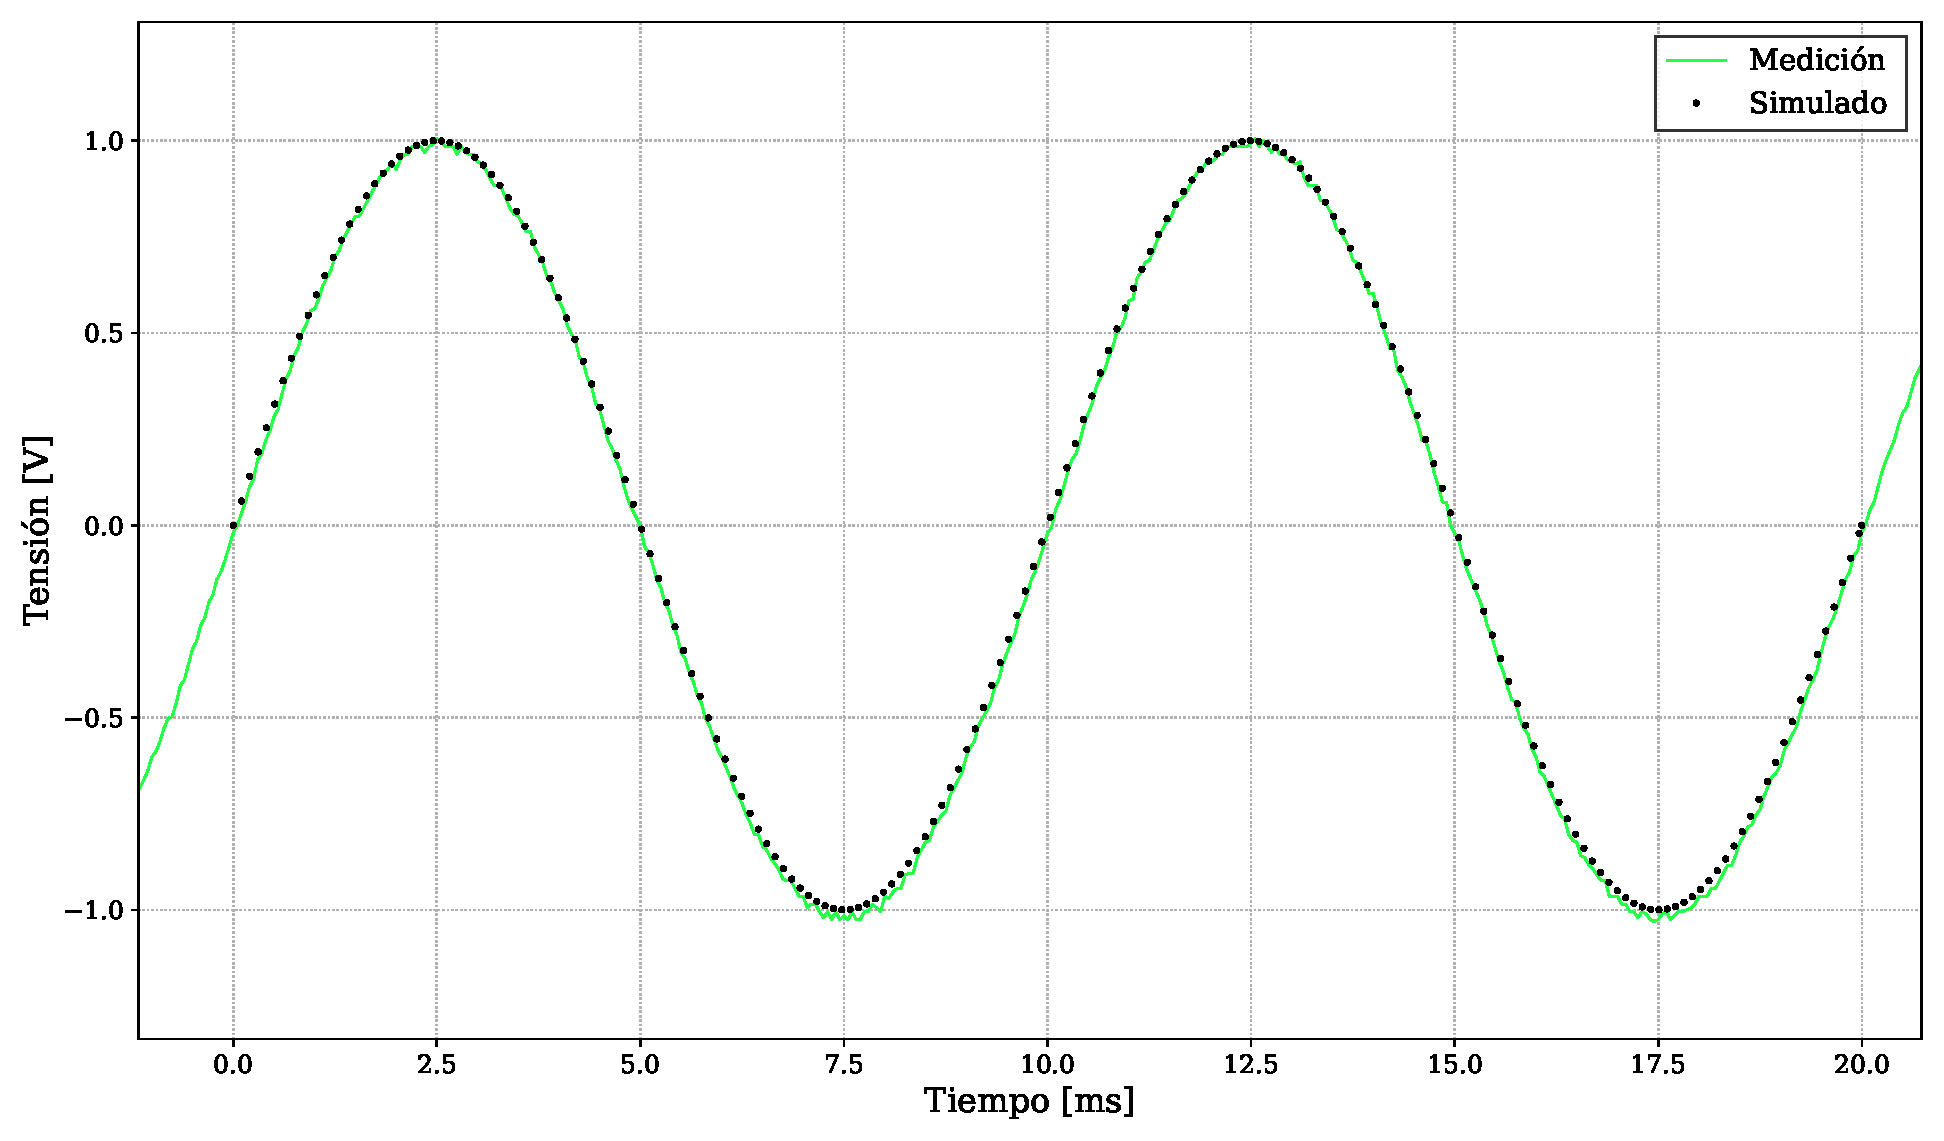
\includegraphics[width=\textwidth]{ej2a_teoprac.pdf} 
        \caption{Comparación de la salida medida con la simulada, circuito de la figura 
        \ref{fig:Ej2buffer} con los parámetros del caso A. La señal simulada es la punteada 
        y la medida es la curva verde.}
        \label{fig:Ej2a}
    \end{minipage}
\end{figure}


\subsection{Caso B}

    \begin{table}[H]
    \centering
    \begin{tabular}{|c|c|c|c|c|c|c|c|}
    \hline
    Caso & $+V_{cc}\ [\text{V}]$ & $-V_{cc}\ [\text{V}]$ & $V_{DC}\ [\text{V}]$ &
    $V_p\ [\text{V}]$ & $f_{in}\ [\text{Hz}]$ & $R_L\ [\Omega]$ & Integrado \\ \hline
    B & 10 & -10 & 0 & 10 & 100 & $\infty$ & LM741 \\ \hline
    \end{tabular}
    \end{table}

    Se compara la salida con la entrada, tanto la medida como la simulada, en las figuras \ref{fig:pdf1} y \ref{fig:pdf2}.
    En principio, el clipping de la salida en ambos casos es esperable, pues al intentar obtener una salida cercana a Vcc+ o Vcc-, 
    los operacionales que no son ''rail to rail'' como los utilizados en este trabajo fallan al acercarse a los rieles y recortan la señal de salida resultando en una saturación por tensión.
    Observar que la salida medida presenta saturación en las tensiones 9,5V y -8,5V, mientras que la salida simulada presenta saturación en las tensiones 8V y -8V.
    Se estima que la diferencia entre la salida medida y la simulada se debe a que el modelo del LM741 utilizado en LTSpice no es exactamente lo que uno utilizará en realidad, y a que
    el circuito interno de LM741 \cite{datasheet_opamp} no es simétrico, por lo que la salida no será necesariamente simétrica.
    
    

\begin{figure}[htbp]
  \centering
  % Primera imagen en PDF
  \begin{minipage}[b]{0.48\textwidth}
    \centering
    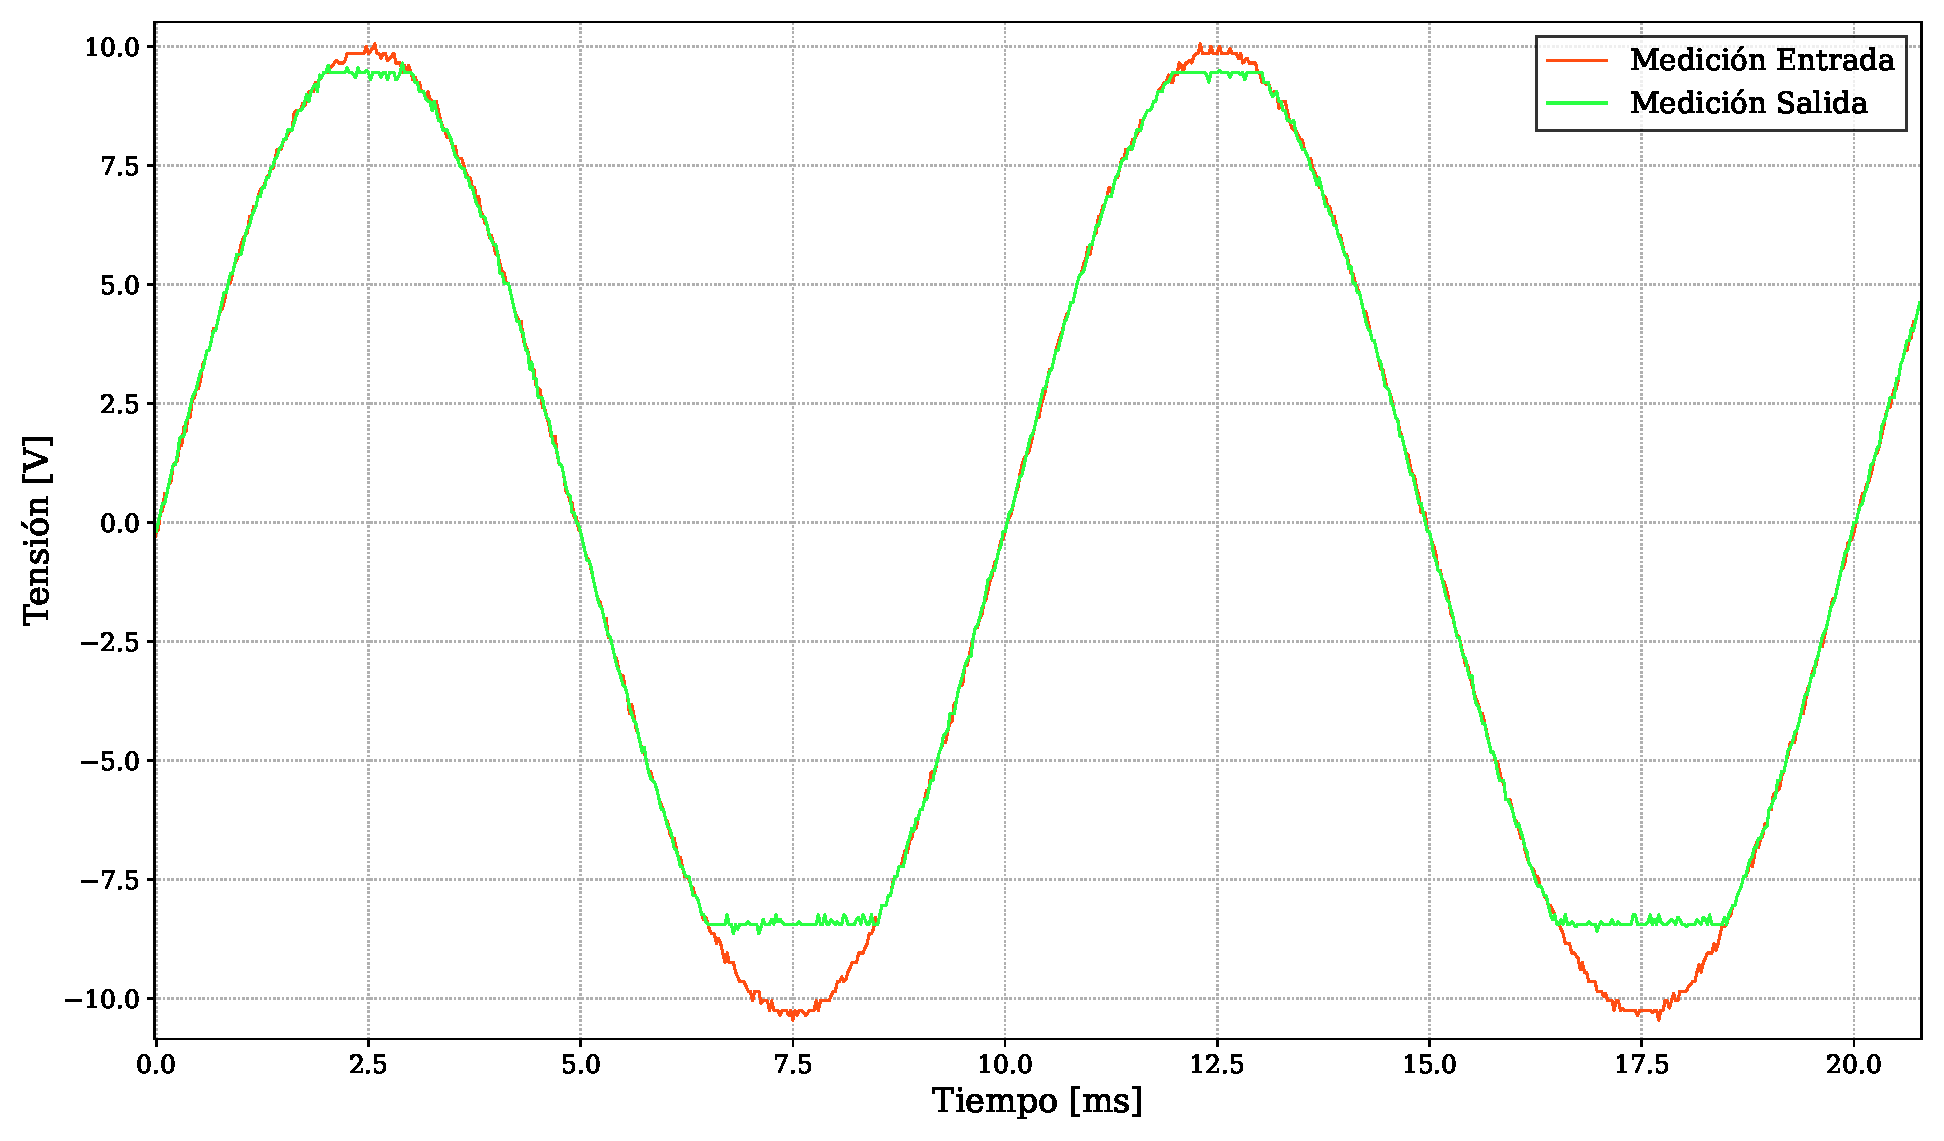
\includegraphics[width=\textwidth]{ej2b_prac.pdf} % Tu archivo PDF
    \caption{Curvas medidas. Vin (rojo) y Vout (verde), las tensiones que presentan clipping a la salida son de 9,5V y -8,5V.}
    \label{fig:pdf1}
  \end{minipage}
  \hfill % Espacio entre imágenes
  % Segunda imagen en PDF
  \begin{minipage}[b]{0.48\textwidth}
    \centering
    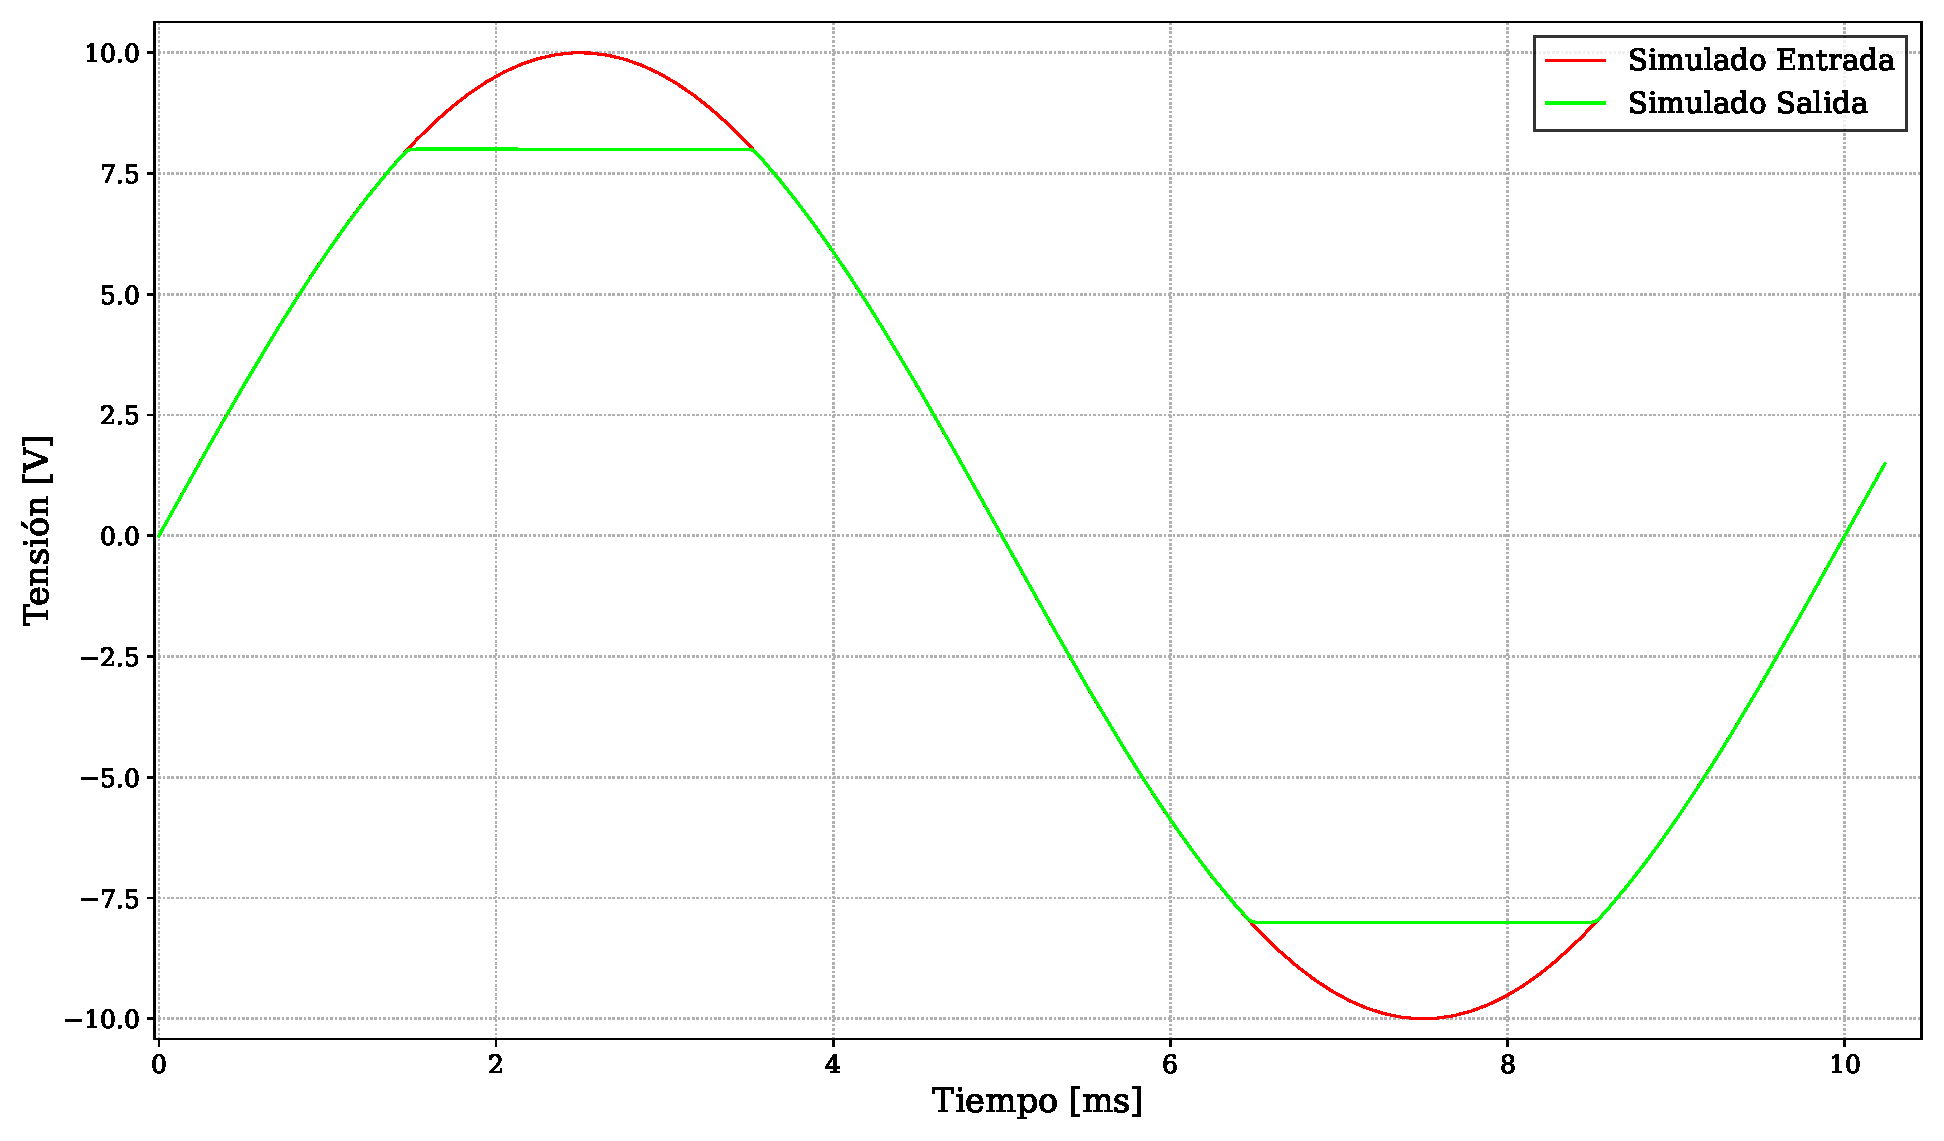
\includegraphics[width=\textwidth]{ej2b_teo.pdf} % Tu archivo PDF
    \caption{Curvas simuladas. Vin (rojo) y Vout (verde), las tensiones que presentan clipping a la salida son de 8V y -8V.}
    \label{fig:pdf2}
  \end{minipage}
\end{figure}



\subsection{Caso C}

    \begin{table}[H]
    \centering
    \begin{tabular}{|c|c|c|c|c|c|c|c|}
    \hline
    Caso & $+V_{cc}\ [\text{V}]$ & $-V_{cc}\ [\text{V}]$ & $V_{DC}\ [\text{V}]$ &
    $V_p\ [\text{V}]$ & $f_{in}\ [\text{Hz}]$ & $R_L\ [\Omega]$ & Integrado \\ \hline
    C & 10 & -2 & 0 & 3 & 100 & $\infty$ & TL072 y LM741 \\ \hline
    \end{tabular}
    \end{table}
\subsubsection{TL072}
Se compara lo medido con lo simulado en las figuras \ref{fig:pdf3} y \ref{fig:pdf4}. 
Primero, note que ambas figuras presentan el comportamiento denominado como Phase Reversal ~\cite{analog_phase_reversal}.
El fenómeno de inversión visto %, 
ocurre cuando la tensión de entrada se va del rango de “Modo Común”, que en el caso del TL072 es de 
(Vcc–)–0.3 V a (Vcc–) + 36 V (obtenido de la datasheet ~\cite{datasheet_tl072}), o  desde -2.3V hasta 34V en este caso. Este fenómeno es
 causado por el apagado de etapas internas del Op. Amp., que ocurre por la pérdida de tensión 
 de polarización de transistores en el interior del integrado. Se ve claramente que aquí
  Vin llega hasta -3V por lo que excede el límite inferior del rango ya mencionado, por lo
   que tiene sentido que ocurra Phase Reversal. Cabe aclarar que el fabricante le avisa al usuario que si se opera al dispositivo fuera de la zona recomendada, el dispositivo no necesariamente funcionará como debe.
    Notar que la tensión a la que llega la 
   sección de la señal de salida con Phase Reversal se mueve directamente hasta el otro
    “riel” o lo que en este caso corresponde a la tensión de saturación positiva. En caso de 
    trabajar con un circuito propenso a sufrir phase reversal se puede implementar un
     circuito de protección contra este efecto.
Ahora, volviendo a la comparación de lo medido con lo simulado, se observa que la salida
 medida presentó saturación en la tensión 9,4V, un valor muy cercano a la tensión de saturación positiva en la simulación (9,5V).
 Sin embargo, sí se puede ver una diferencia más fuerte en la tensión de saturación negativa, que en la medición es de -1,7V y en la simulación es de -0,5V.
La causa más probable es la diferencia entre el modelo del Op Amp. utilizado en LTSpice y el integrado real. Como se vio en el caso B con el LM741,
se veía una diferencia en la tensión de saturación negativa entre la simulación y la medición, pero en ambos casos la simulación se aproxima lo suficiente a la medición para considerar que el circuito cumple con lo esperado desde el punto de vista práctico.
 
\begin{figure}[htbp]
  \centering
  % Primera imagen en PDF
  \begin{minipage}[b]{0.48\textwidth}
    \centering
    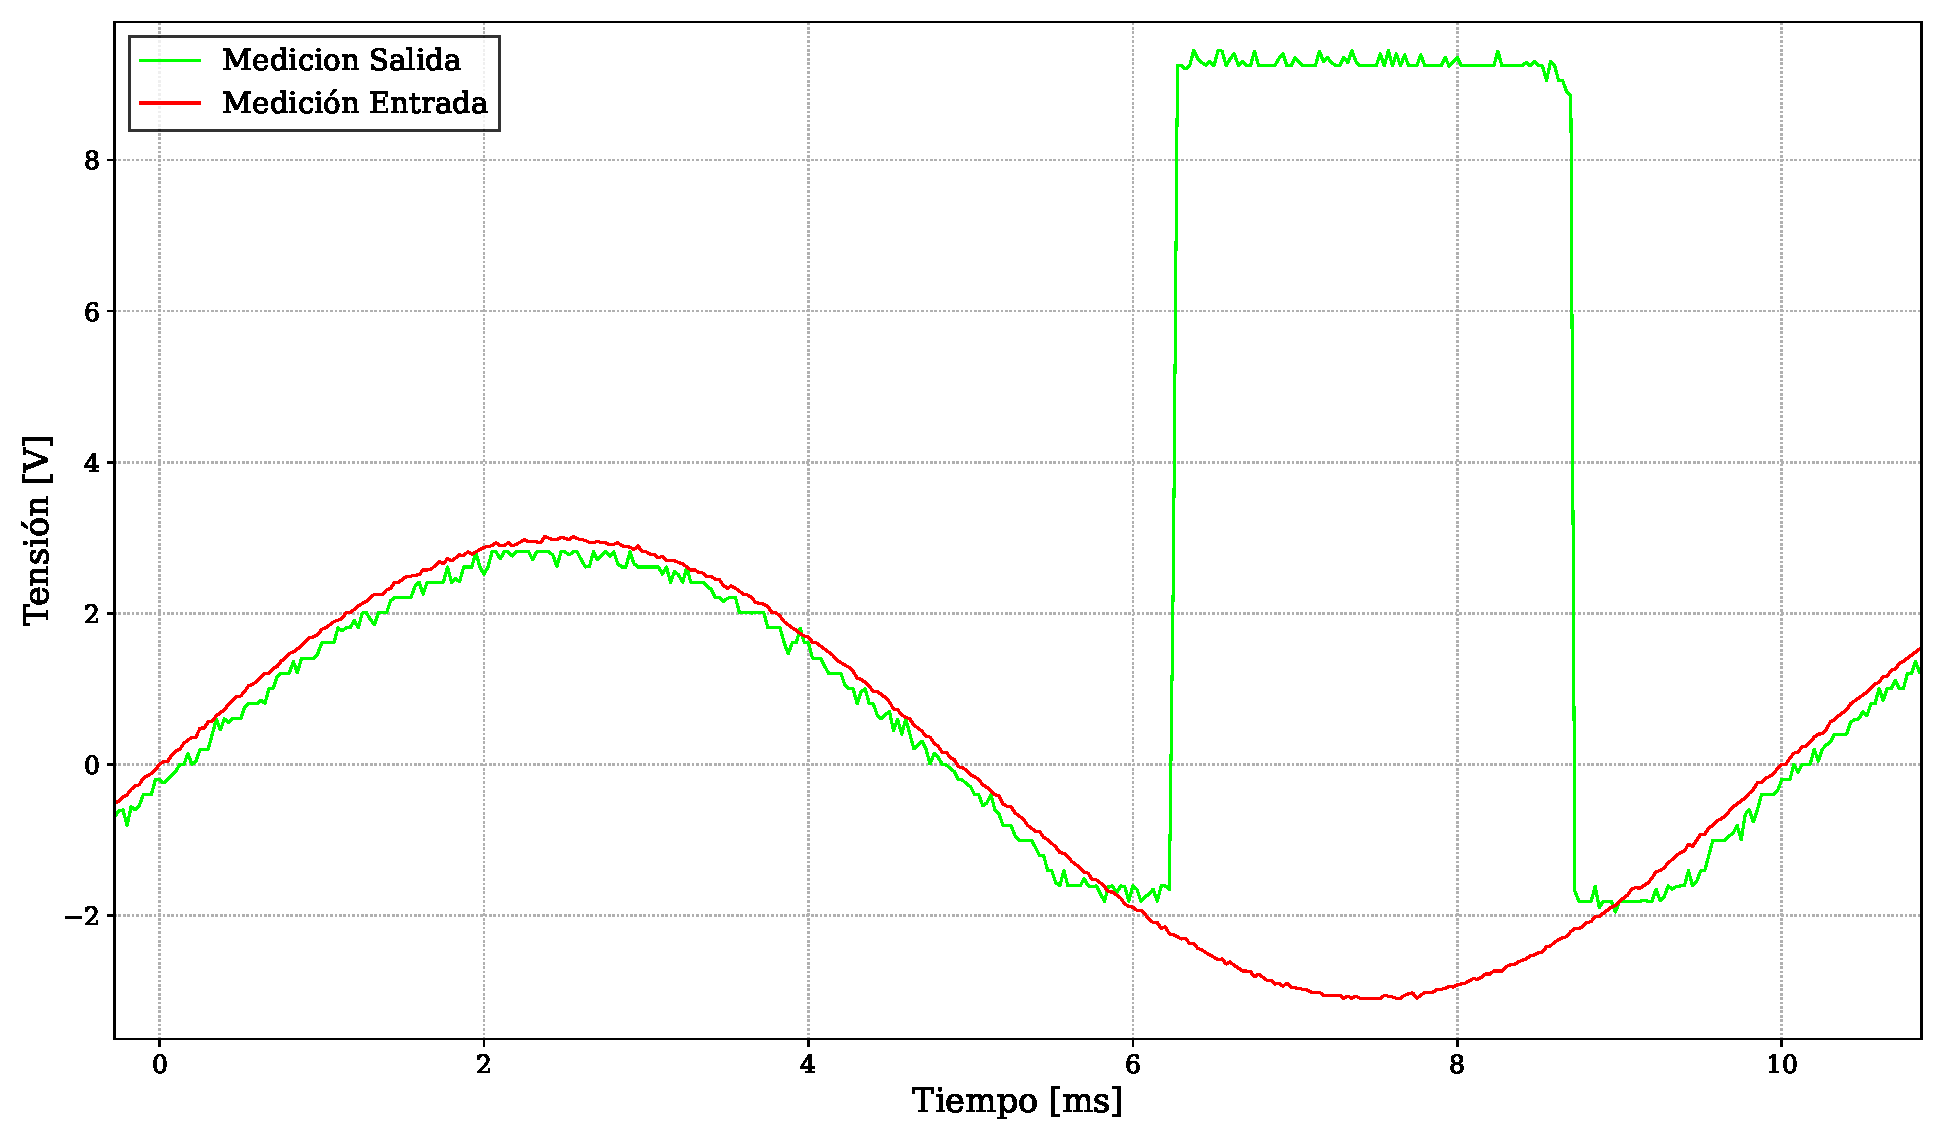
\includegraphics[width=\textwidth]{ej2c_prac.pdf} % Tu archivo PDF
    \caption{Curvas medidas. Vin (rojo) y Vout (verde), las tensiones que presentan clipping a la salida son de 9,5V y -1,7V.}
    \label{fig:pdf3}
  \end{minipage}
  \hfill % Espacio entre imágenes
  % Segunda imagen en PDF
  \begin{minipage}[b]{0.48\textwidth}
    \centering
    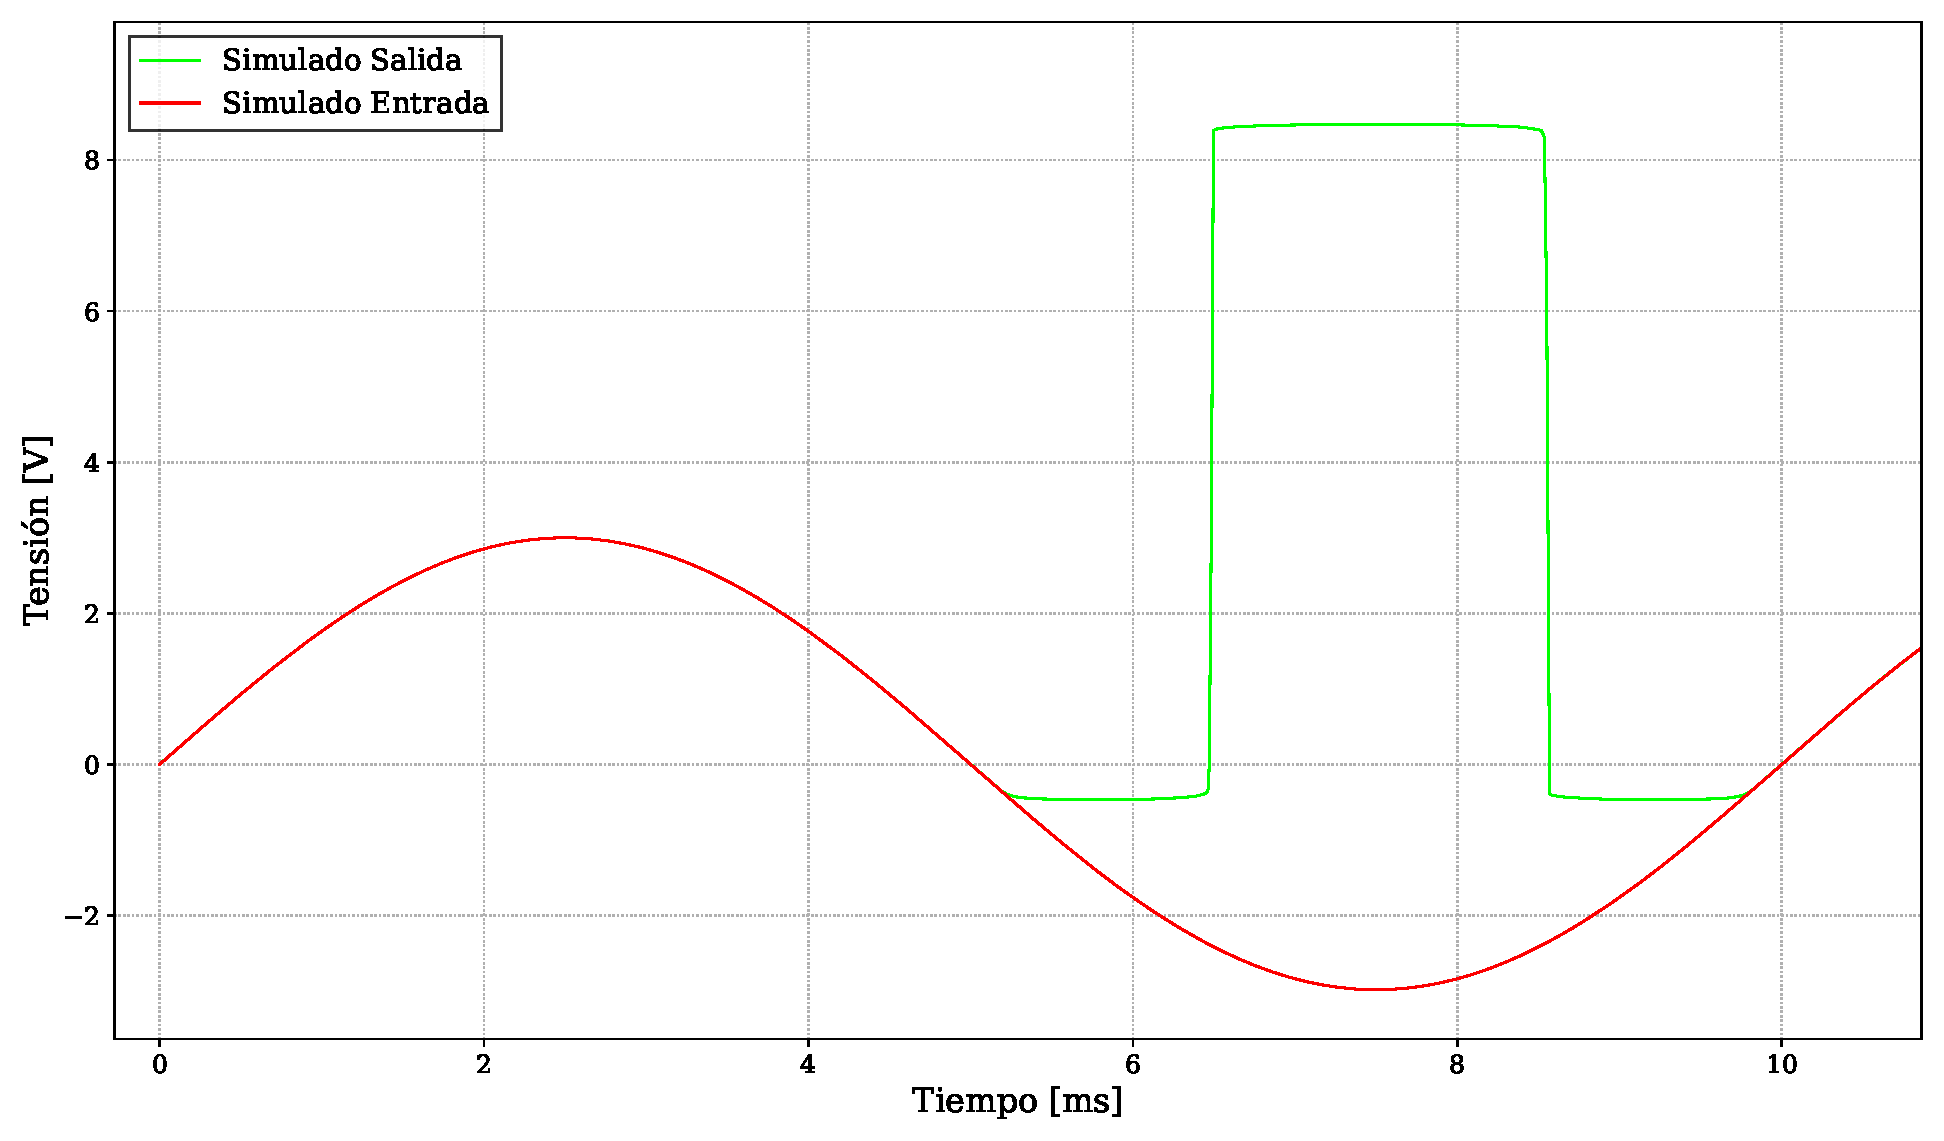
\includegraphics[width=\textwidth]{ej2c_teo.pdf} % Tu archivo PDF
    \caption{Curvas simuladas. Vin (rojo) y Vout (verde), las tensiones que presentan clipping a la salida son de -0,5V y 8,5V.}
    \label{fig:pdf4}
  \end{minipage}
\end{figure}

\subsubsection{LM741}
Se compara nuevamente lo simulado con lo medido en las figuras \ref{fig:pdf5} y \ref{fig:pdf6}. Notar que hay diferencia entre tensiones de saturación negativa, 
además de que no hay Phase Reversal en este caso. 
En principio el hecho de que no haya Phase Reversal se puede deber a que no es un fenómeno esperable en 
un dispositivo 
que se basa en transistores bipolares a diferencia de los dispositivos que sí implementan transistores del tipo JFET (comentado en ~\cite{analog_phase_reversal}), se lo puede verificar viendo el esquema interno del LM741 en su datasheet.
Luego, la diferencia de tensiones de saturación negativa se puede deber a el modelo Spice del Op. Amp.. Se notó que incluso el modelo Spice
 parece realizar la simple operación de (Vcc+)-2V y (Vcc-)+2V para fijar las tensiones 
 de saturación positiva y negativa respectivamente. Esto se verificó con un par de valores
  de Vcc+ y Vcc- distintos colocando en la entrada una señal que exceda el rango de 
  alimentación y así forzando la saturación, el lector podrá observarlo en la figura \ref{fig:curiosidad2}, ubicada en el anexo. 
\begin{figure}[htbp]
  \centering
  % Primera imagen en PDF
  \begin{minipage}[b]{0.48\textwidth}
    \centering
    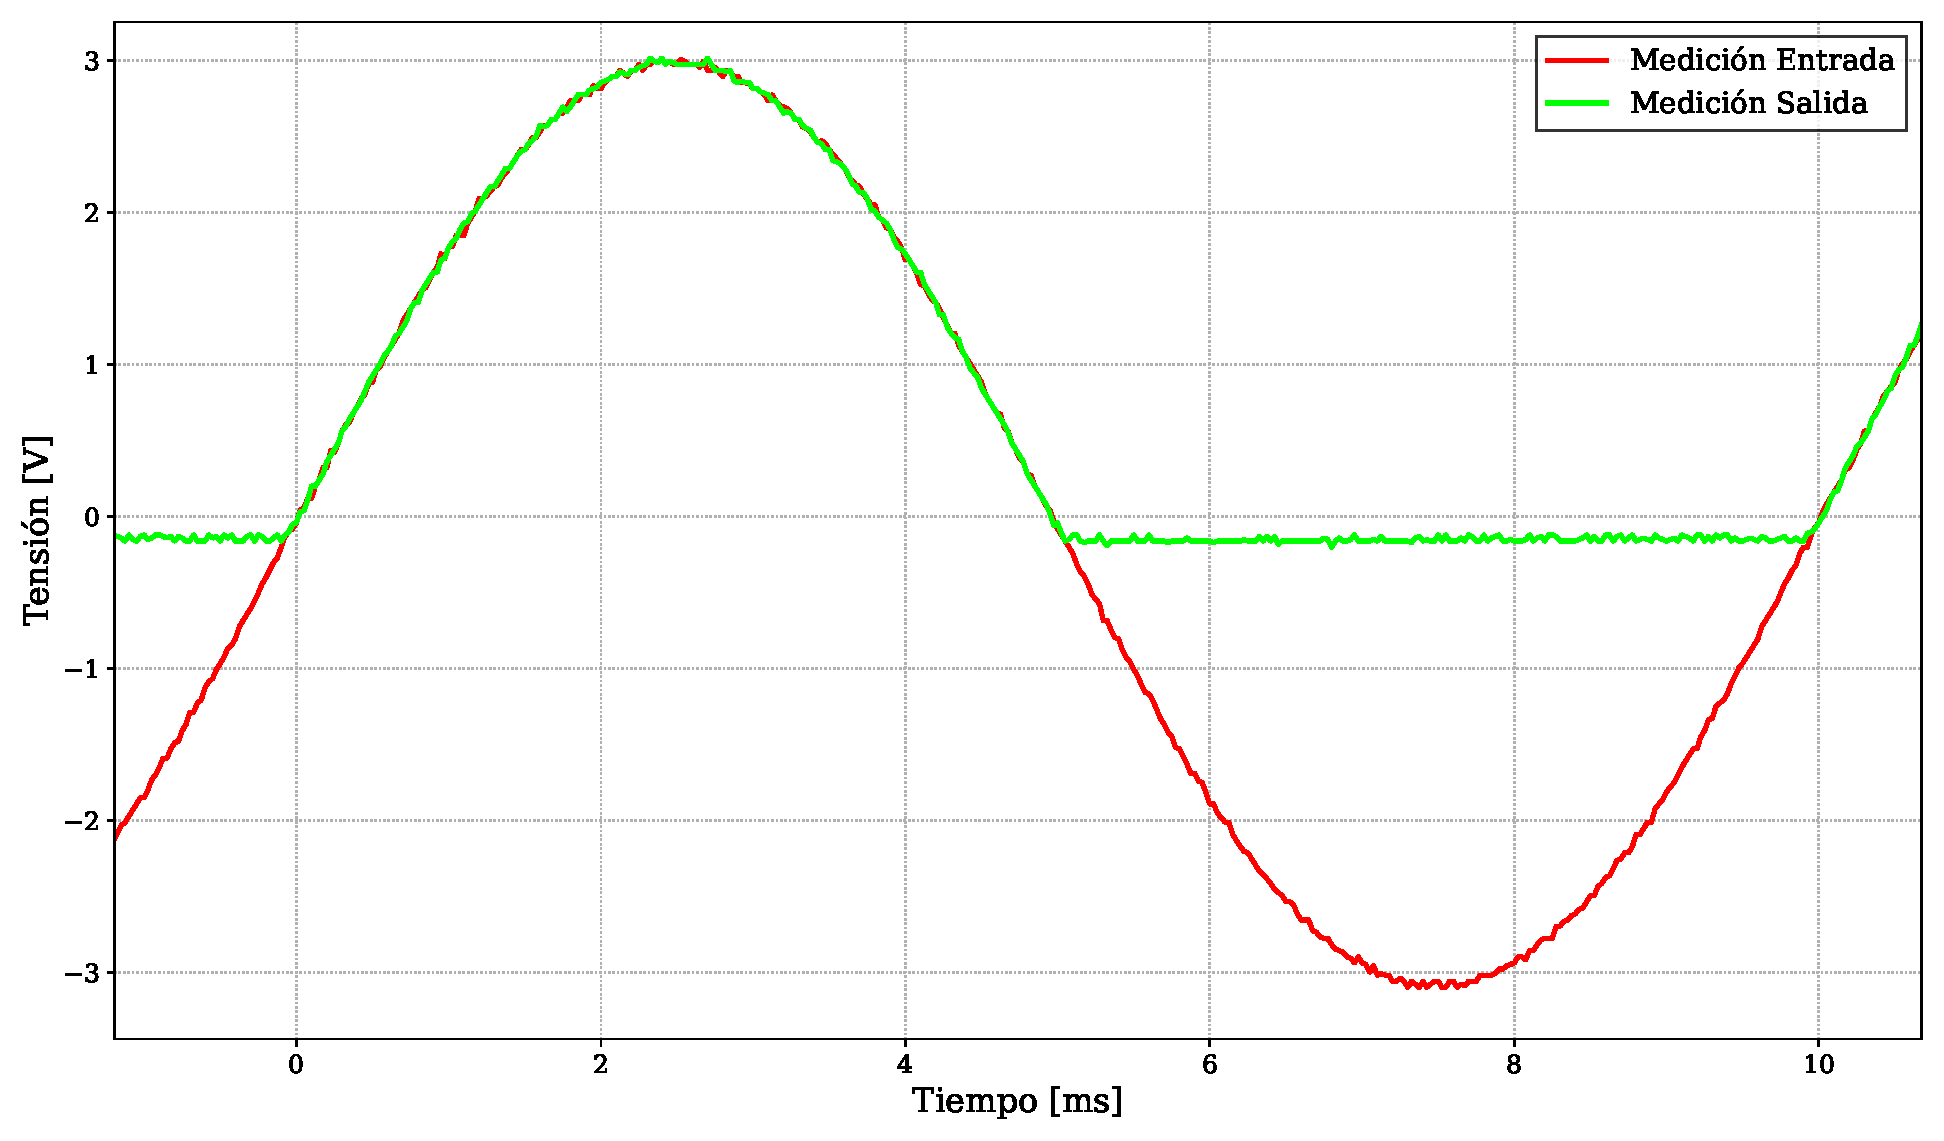
\includegraphics[width=\textwidth]{ej2cLM_prac.pdf} % Tu archivo PDF
    \caption{Curvas medidas. Vin (rojo) y Vout (verde), la tensión que presenta clipping a la salida es de -0.16V.}
    \label{fig:pdf5}
  \end{minipage}
  \hfill % Espacio entre imágenes
  % Segunda imagen en PDF
  \begin{minipage}[b]{0.48\textwidth}
    \centering
    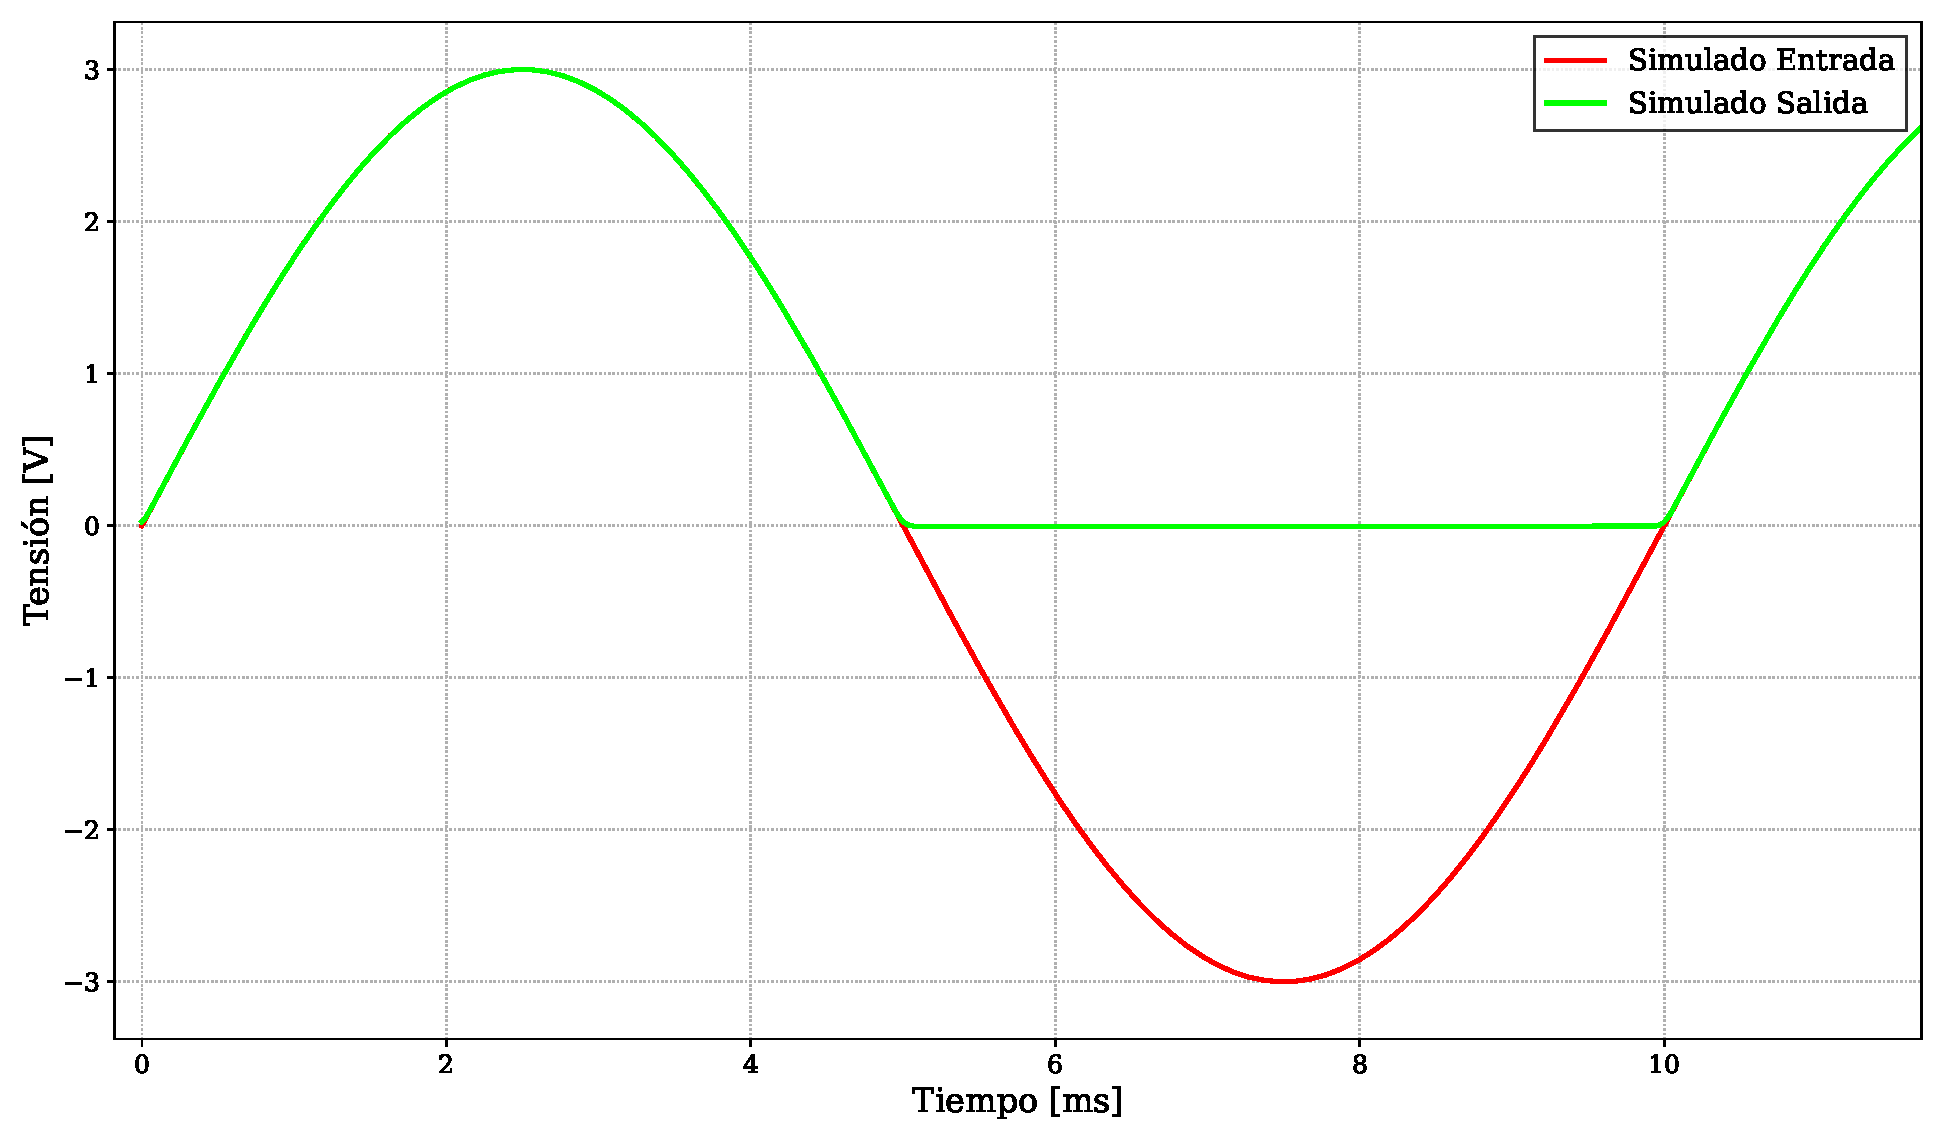
\includegraphics[width=\textwidth]{ej2cLM_teo.pdf} % Tu archivo PDF
    \caption{Curvas simuladas. Vin (rojo) y Vout (verde), la tensión que presenta clipping a la salida es de 0V.}
    \label{fig:pdf6}
  \end{minipage}
\end{figure}

%%%%

\subsection{Caso D}

    \begin{table}[H]
\centering
\begin{tabular}{|c|c|c|c|c|c|c|c|}
\hline
Caso & $+V_{cc}\ [\text{V}]$ & $-V_{cc}\ [\text{V}]$ & $V_{DC}\ [\text{V}]$ &
 $V_p\ [\text{V}]$ & $f_{in}\ [\text{Hz}]$ & $R_L\ [\Omega]$ & Integrado \\ \hline
D & 4 & -4 & 3.5 & 1 & 100 & $\infty$ & TL072 \\ \hline
\end{tabular}
\end{table}
Comparando la salida medida con la simulada en las figuras \ref{fig:pdf7} y \ref{fig:pdf8}, se observa que la salida medida presenta saturación en la tensión 3,5V, mientras que la salida simulada presenta saturación en las tensiones 2,42V y 2,48V.
Esta diferencia se la atribuye al modelo de Spice de TL082 utilizado. Se puede comprobar que si no fuera porque el modelo simulado no es exacto al simular las tensiones de saturación, las curvas obtenidas serían más fieles a la realidad, como se ve en la figura \ref{fig:curiosidad}, donde se simula el mismo circuito pero con Vcc+ = 5V y Vcc- = -5V,
 y se observa que la salida simulada presenta saturación en la tensión 3,5V, como lo visto en la curva medida. Notar que la ''corrección'' aplicada no es suficiente para que la salida simulada sea igual a la medida, se puede ver en las curvaturas de la salida cuando la entrada se acerca o se aleja de la tensión de saturación en la figura \ref{fig:curiosidad}.
\begin{figure}[htbp]
  \centering
  % Primera imagen en PDF
  \begin{minipage}[b]{0.48\textwidth}
    \centering
    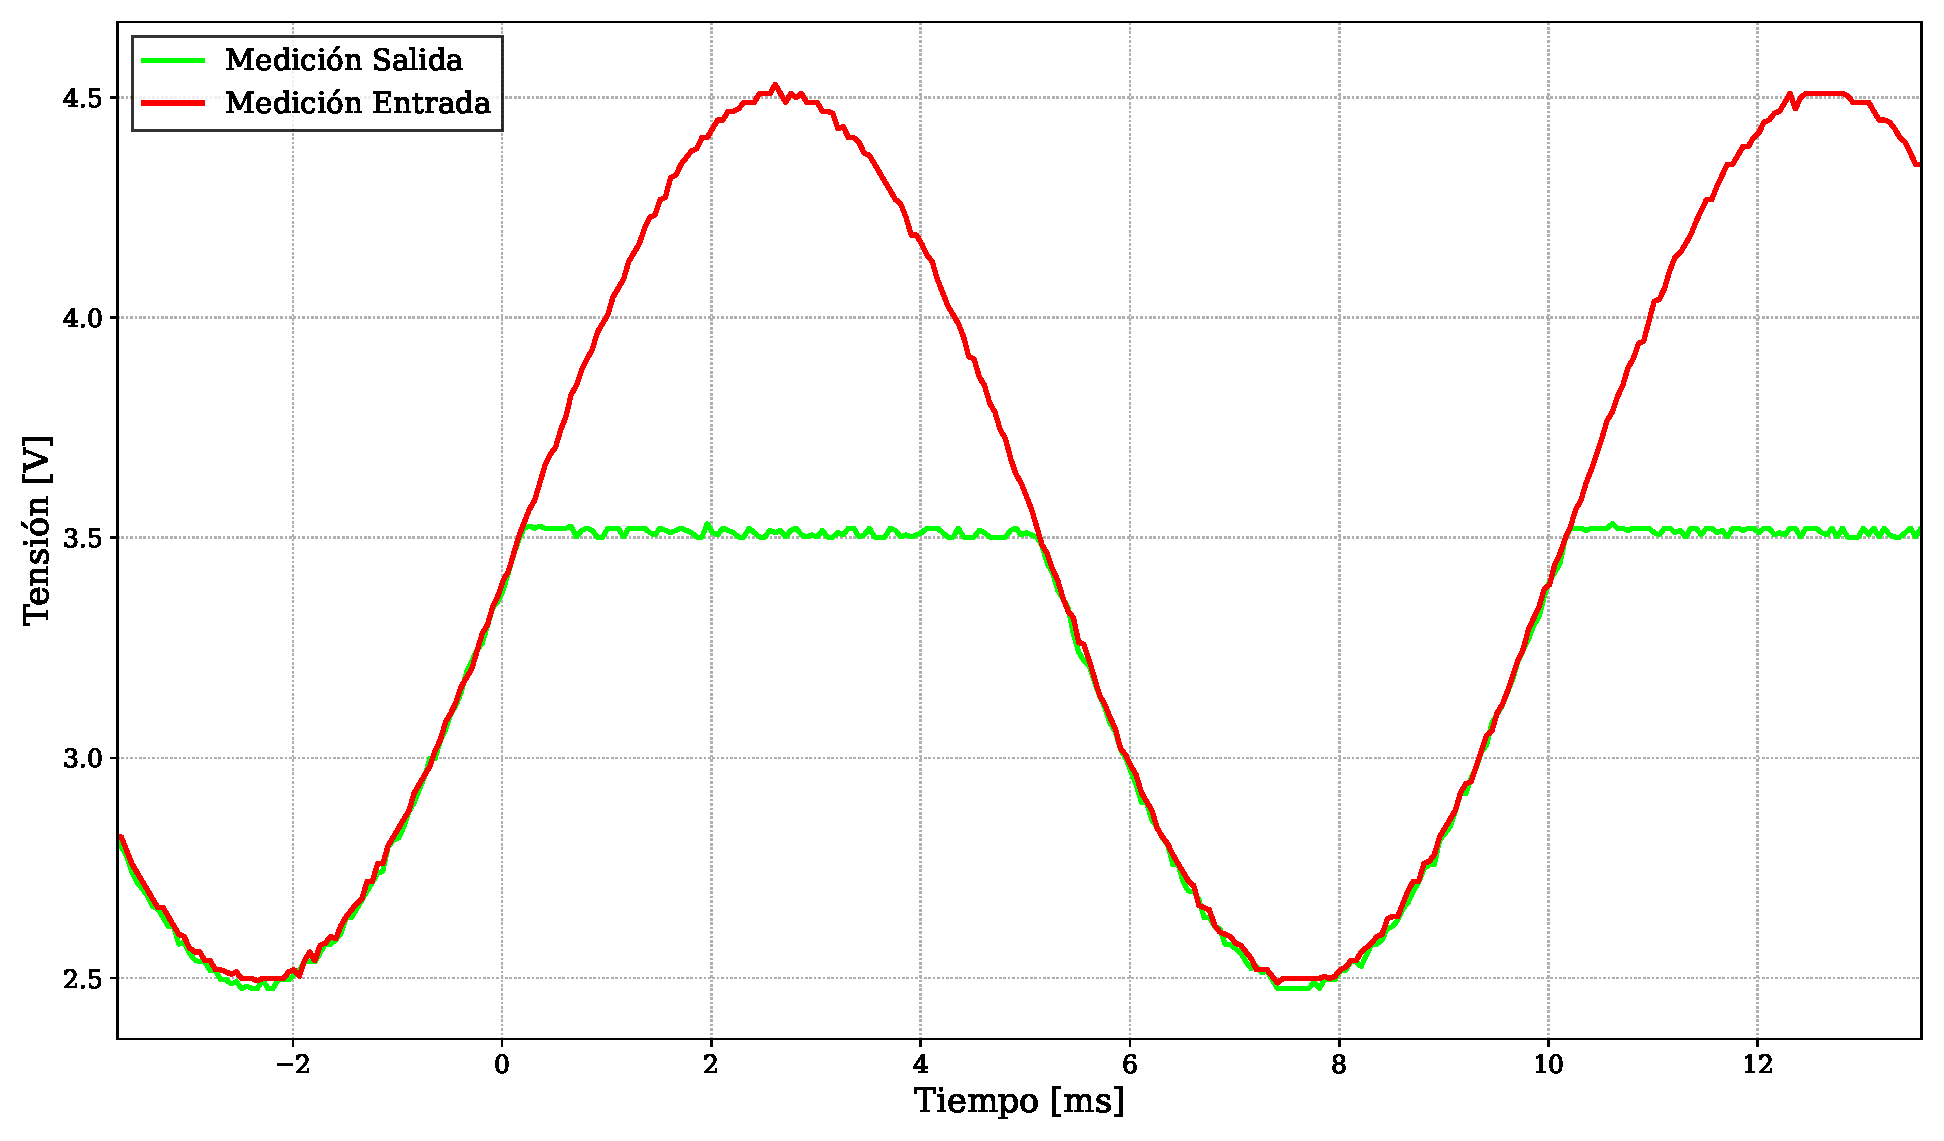
\includegraphics[width=\textwidth]{ej2d_prac.pdf} % Tu archivo PDF
    \caption{Curvas medidas. Vin (rojo) y Vout (verde), la tensión que presenta clipping a la salida es de 3,5V.}
    \label{fig:pdf7}
  \end{minipage}
  \hfill % Espacio entre imágenes
  % Segunda imagen en PDF
  \begin{minipage}[b]{0.48\textwidth}
    \centering
    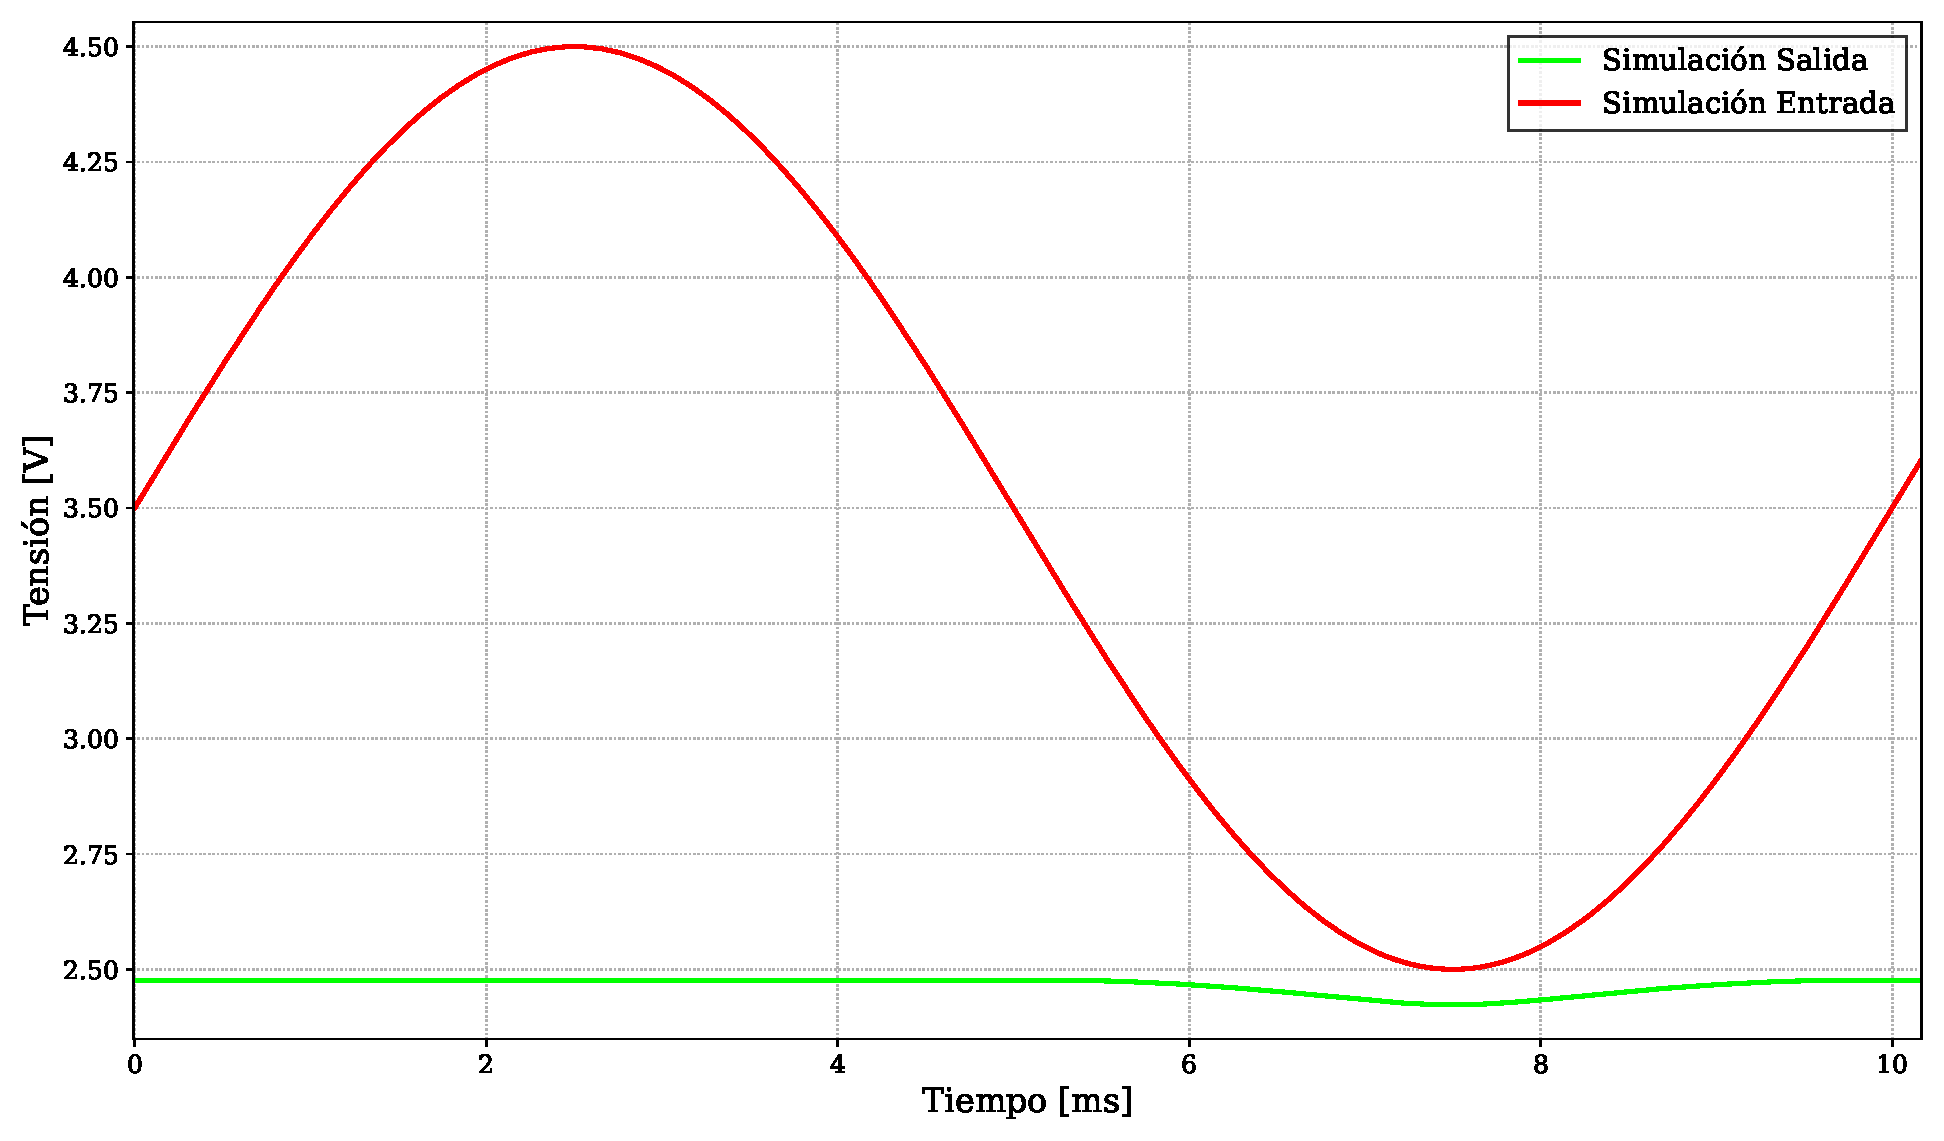
\includegraphics[width=\textwidth]{ej2d_teo.pdf} % Tu archivo PDF
    \caption{Curvas simuladas. Vin (rojo) y Vout (verde), la tensión que presenta clipping a la salida en torno a 2,4V (minimo en 2,42V y máximo en 2,48V).}
    \label{fig:pdf8}
  \end{minipage}
\end{figure}

\begin{figure}[htbp]
    \centering
    % Ajusta el ancho con respecto al texto (ej. 80% del ancho del texto)
    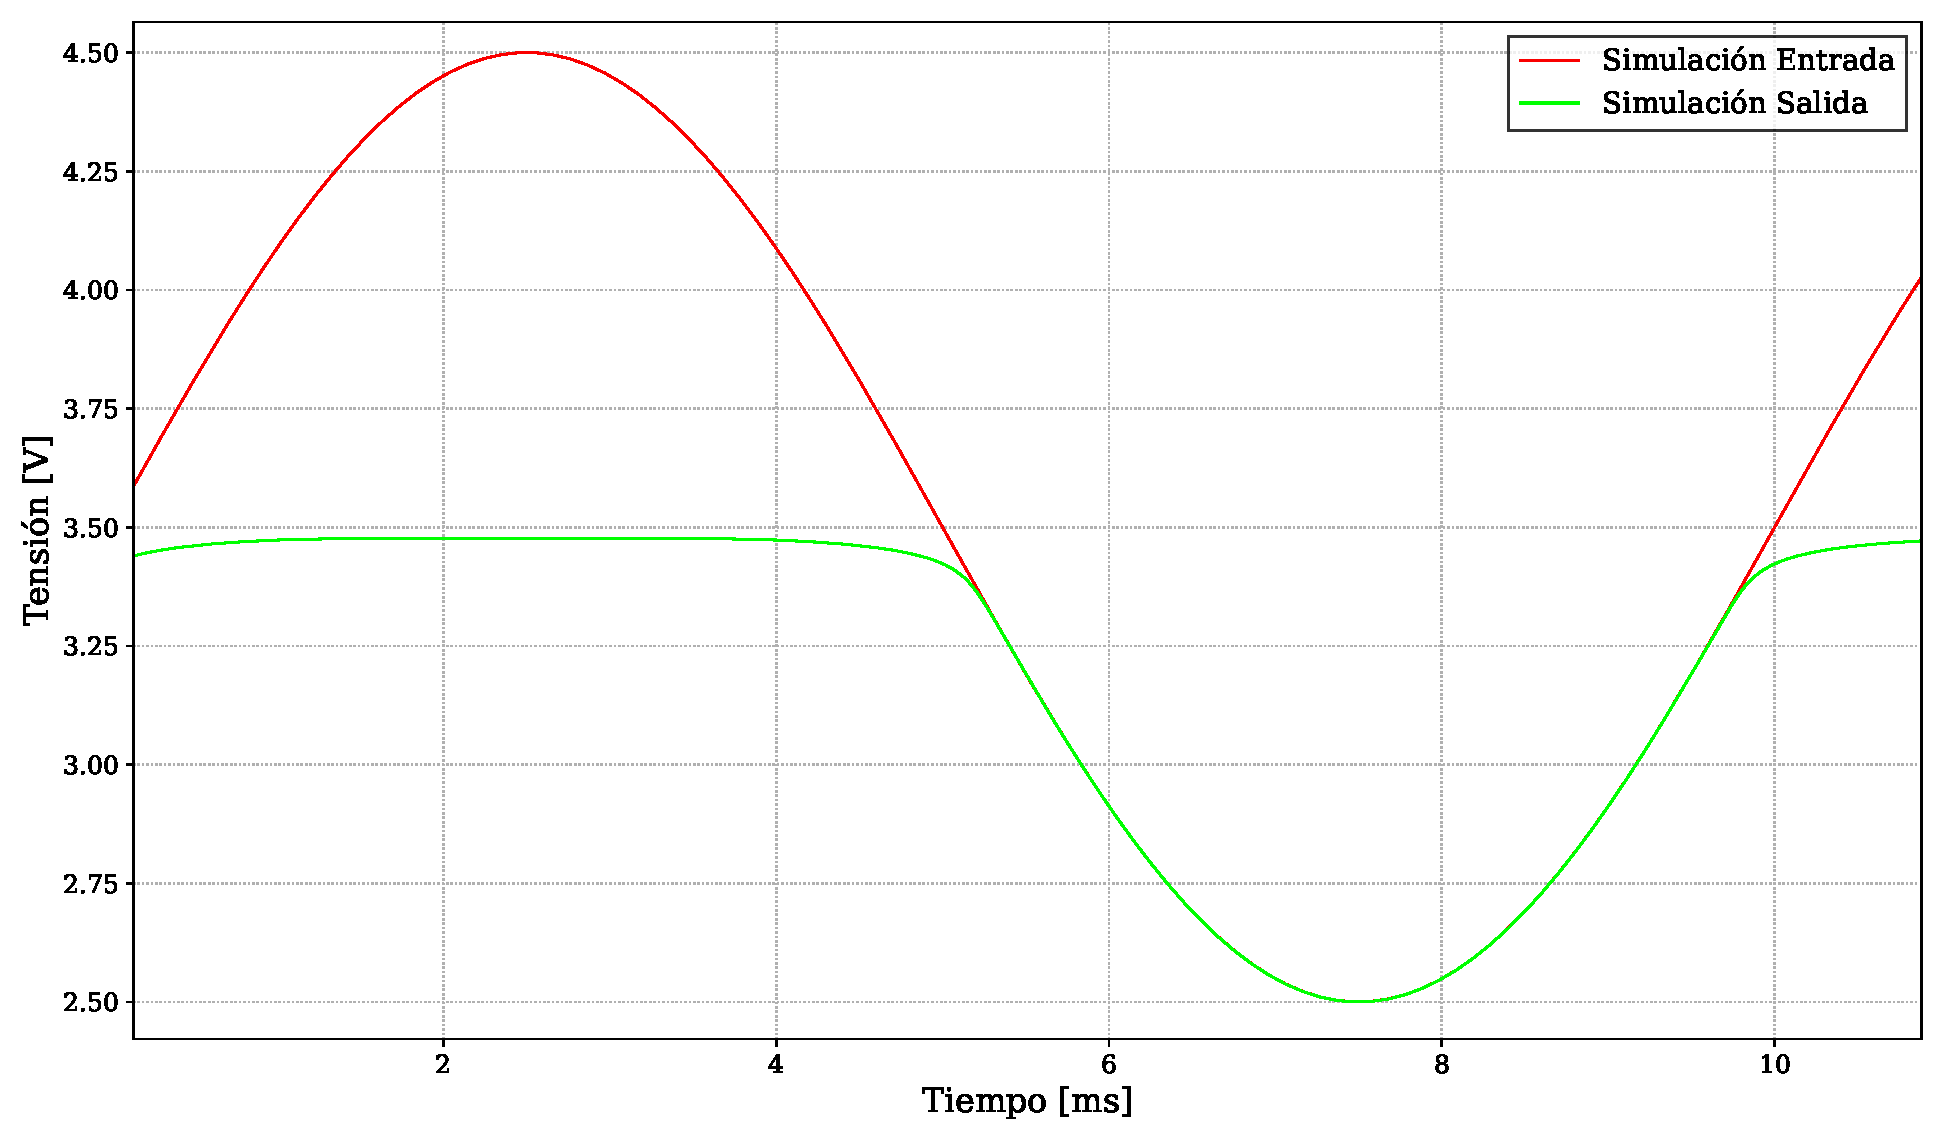
\includegraphics[width=0.6\textwidth]{ej2d_teo5V.pdf} 
    \caption{Curvas simuladas con Vcc+ = 5V y Vcc- = -5V. Vin (rojo) y Vout (verde), la tensión que presenta clipping a la salida en 3,5V, como lo visto en la curva medida. Observe las curvaturas de la salida al momento de salir/entrar en saturación.}
    \label{fig:curiosidad}
\end{figure}
\vspace{2cm}
\subsection{Caso E}
   \begin{table}[H]
\centering
\begin{tabular}{|c|c|c|c|c|c|c|c|}
\hline
Caso & $+V_{cc}\ [\text{V}]$ & $-V_{cc}\ [\text{V}]$ & $V_{DC}\ [\text{V}]$ &
 $V_p\ [\text{V}]$ & $f_{in}\ [\text{Hz}]$ & $R_L\ [\Omega]$ & Integrado \\ \hline
E & 10 & -10 & 0 & 5 & 100 & 100 & TL072 \\ \hline
\end{tabular}
\end{table}
    
En este caso en particular, observar que el circuito tiene una resistencia de carga relativamente baja, por lo que es esperable que 
la salida se vea influenciada por la corriente que debe entregar el Op. Amp. para poder mantener la salida en la tensión deseada.
Notar que, tal como se ve en la figura 5-12 de la datasheet (\ref{fig:pdf40}), la corriente de salida máxima hasta la que el dispositivo mantiene la tensión de salida estable, es de aproximadamente 26mA.
 Análogamente se aplica el mismo razonamiento con la figura 5-13 (\ref{fig:pdf41}) de la misma datasheet. 
Se deduce entonces, que la tensión máxima de salida esperable es de aproximadamente $\pm$2,6V, esto se puede ver en las figuras \ref{fig:pdf9} y \ref{fig:pdf10} (como la carga es de 100$\Omega$, se deduce que las corrientes que soporta el Op. Amp. en su salida son de 30mA y -24mA). Notar que como se ya se vio en casos anteriores, si no fuera porque la carga demanda mucha corriente, la tensión pico dada las tensiones Vcc+ y Vcc- alcanzaría la amplitud total de la señal de entrada.
\begin{figure}[htbp]
  \centering
  % Primera imagen en PDF
  \begin{minipage}[b]{0.48\textwidth}
    \centering
    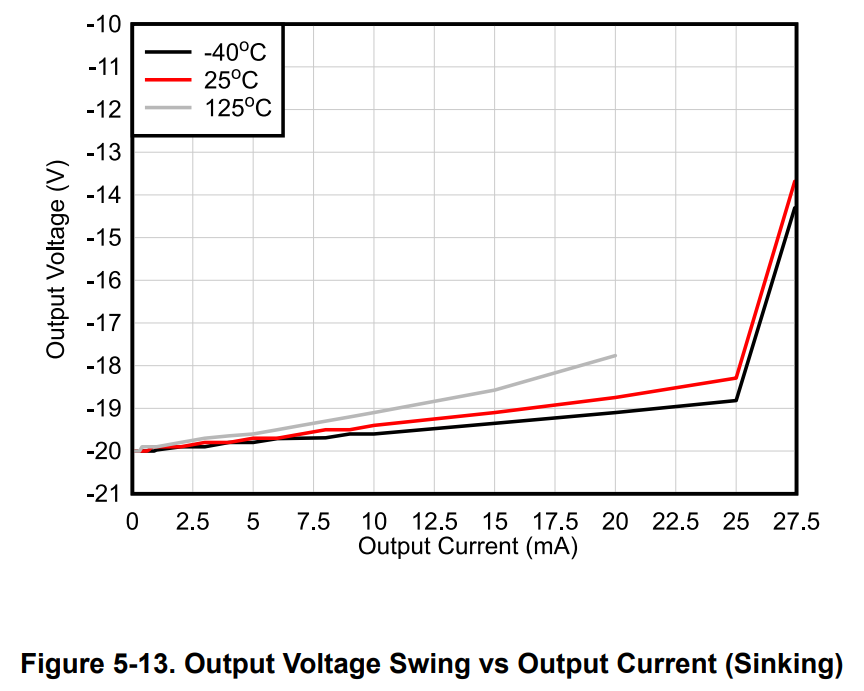
\includegraphics[width=\textwidth]{fig5-13.png} % Tu archivo PDF
    \caption{Curvas informadas de TL072 en su datasheet. Notar que la corriente máxima que logra ''absorber'' el dispositivo sin desestabilizar su salida es de $\approx 26mA$}
    \label{fig:pdf41}
  \end{minipage}
  \hfill % Espacio entre imágenes
  % Segunda imagen en PDF
  \begin{minipage}[b]{0.48\textwidth}
    \centering
    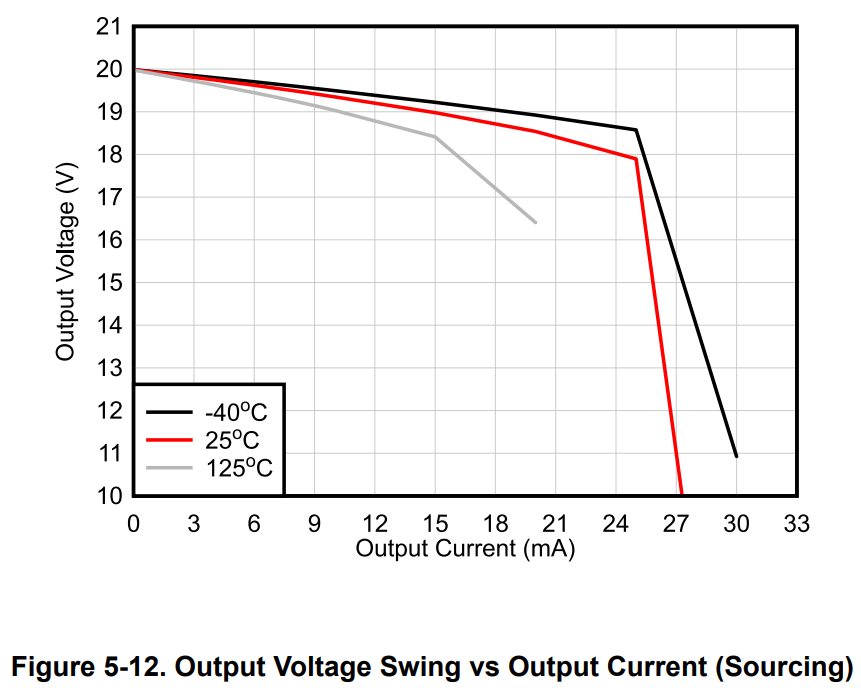
\includegraphics[width=\textwidth]{fig5-12.png} % Tu archivo PDF
    \caption{Curvas informadas de TL072 en su datasheet. Notar que la corriente máxima que logra entregar el dispositivo sin desestabilizar su salida es de $\approx 26mA$}
    \label{fig:pdf40}
  \end{minipage}
\end{figure}



\begin{figure}[htbp]
  \centering
  % Primera imagen en PDF
  \begin{minipage}[b]{0.48\textwidth}
    \centering
    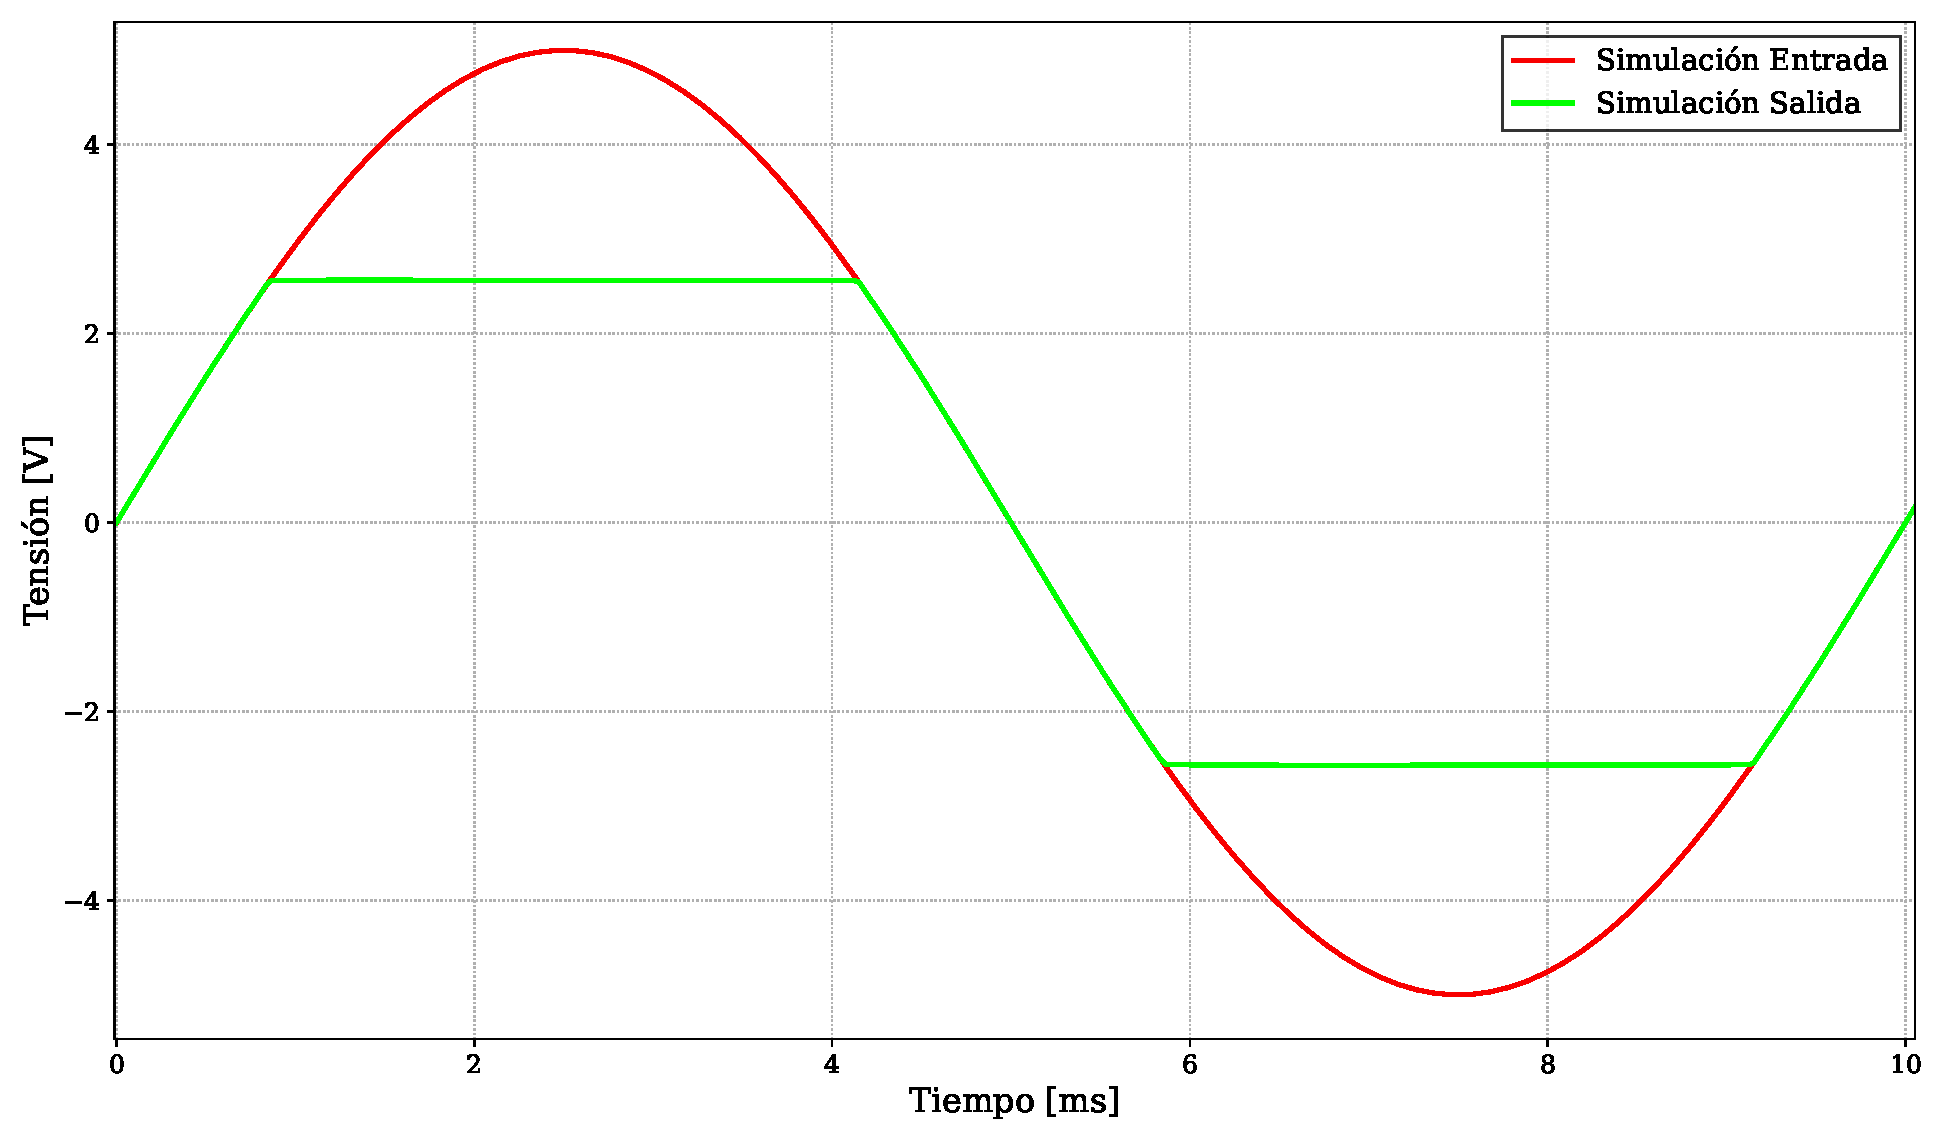
\includegraphics[width=\textwidth]{ej2e_teo.pdf} % Tu archivo PDF
    \caption{Curvas simuladas. Vin (rojo) y Vout (verde), la tensión que presenta clipping a la salida es de $\pm $2,56V.}
    \label{fig:pdf9}
  \end{minipage}
  \hfill % Espacio entre imágenes
  % Segunda imagen en PDF
  \begin{minipage}[b]{0.48\textwidth}
    \centering
    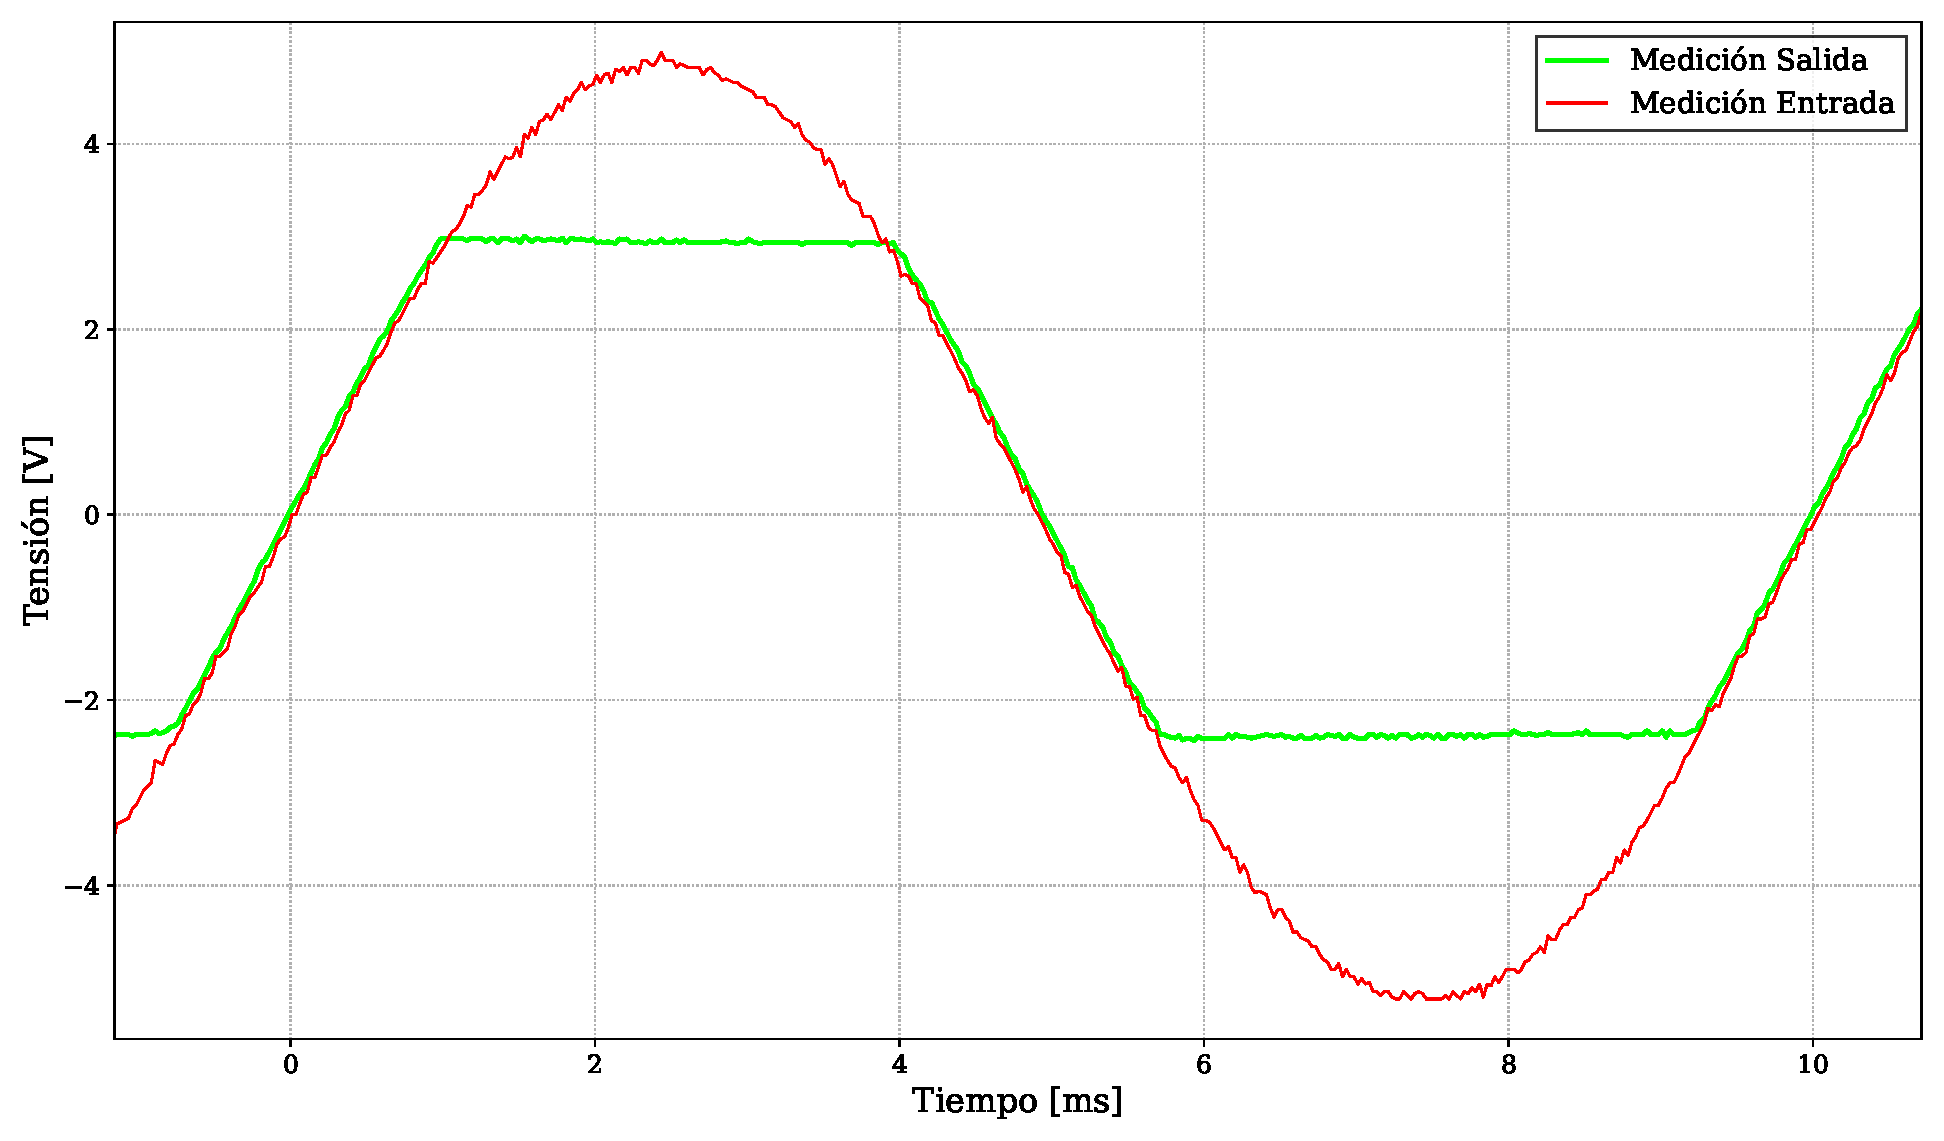
\includegraphics[width=\textwidth]{ej2e_prac.pdf} % Tu archivo PDF
    \caption{Curvas medidas. Vin (rojo) y Vout (verde), la tensión que presenta clipping a la salida en -2,4V y 3V.}
    \label{fig:pdf10}
  \end{minipage}
\end{figure}


\subsection{Caso F}

 \begin{table}[H]
\centering
\begin{tabular}{|c|c|c|c|c|c|c|c|}
\hline
Caso & $+V_{cc}\ [\text{V}]$ & $-V_{cc}\ [\text{V}]$ & $V_{DC}\ [\text{V}]$ &
 $V_p\ [\text{V}]$ & $f_{in}\ [\text{Hz}]$ & $R_L\ [\Omega]$ & Integrado \\ \hline
F & 10 & -10 & 0 & 10 & 100 & 560 & LM741 \\ \hline
\end{tabular}
\end{table}

Notar que la resistencia de carga no es tan baja como en el caso anterior, esto 
posibilita que el caso B y F tengan resultados de simulación idénticos. Ahora bien, lo medido sí muestra diferencias claras con el caso B en cuanto a
 tensiones de clipping a la salida, se observa que: en el caso B, son 9,5V y 8,5V; en el caso F, son 7,9V y -7V. 
 Ver figuras \ref{fig:pdf11} y \ref{fig:pdf12}. Una posible explicación a esto es que al saturarse la ganancia cae y por lo tanto se pierde 
 la propiedad de ''masa virtual'' que aseguraba que las terminales de entrada del Op. Amp. tengan tensiones muy similares.
 Luego, con el operacional saturado, se podría llegar a modelar a la salida del dispositivo como una fuente de tensión real cuya tensión es la de saturación sin carga (ya vista en el caso B)
  con una resistencia en serie denominada $r_o$, y luego la resistencia de carga en serie. 
  Si se considera que la terminal inversora del operacional no consume corriente se podría decir que
   la salida que se medirá del circuito
  corresponde a la salida del divisor resistivo conformado por la resistencia $r_o$ y la de carga.
   A continuación se intenta comprobar esta explicación, despejando la $r_o$ de la expresión 
   $V_{out}=\frac{R_L}{R_L+r_o}\cdot V_{sat\cdot Caso\cdot B}$. 
   Se obtiene que $r_o=113\Omega$, con $V_{out}=7,9V$, $R_L=560\Omega$ y $V_{sat\cdot Caso\cdot B}=9,5V$. El resultado de $r_o$ es de un orden esperable, si bien en el datasheet del LM741 no se encontró ningún valor
   estimado de dicho parámetro, en el caso del TL072 sí se informa, y es alrededor de $125\Omega$, muy cerca del valor obtenido en este caso.
   El hecho de que esta diferencia no se vea en la simulación se puede deber a que el modelo no considera ninguna resistencia de salida como $r_o$, por lo que no importa qué carga tenga el circuito, mientras la corriente exigida por la carga sea menor a la de saturación de 25mA (denominada como Output short circuit current en la datasheet) y la salida no se pase del rango (Vcc+)-2 a (Vcc-)+2, la salida será la esperada idealmente ($r_o=0 \Omega$).
\begin{figure}[htbp]
  \centering
  % Primera imagen en PDF
  \begin{minipage}[b]{0.48\textwidth}
    \centering
    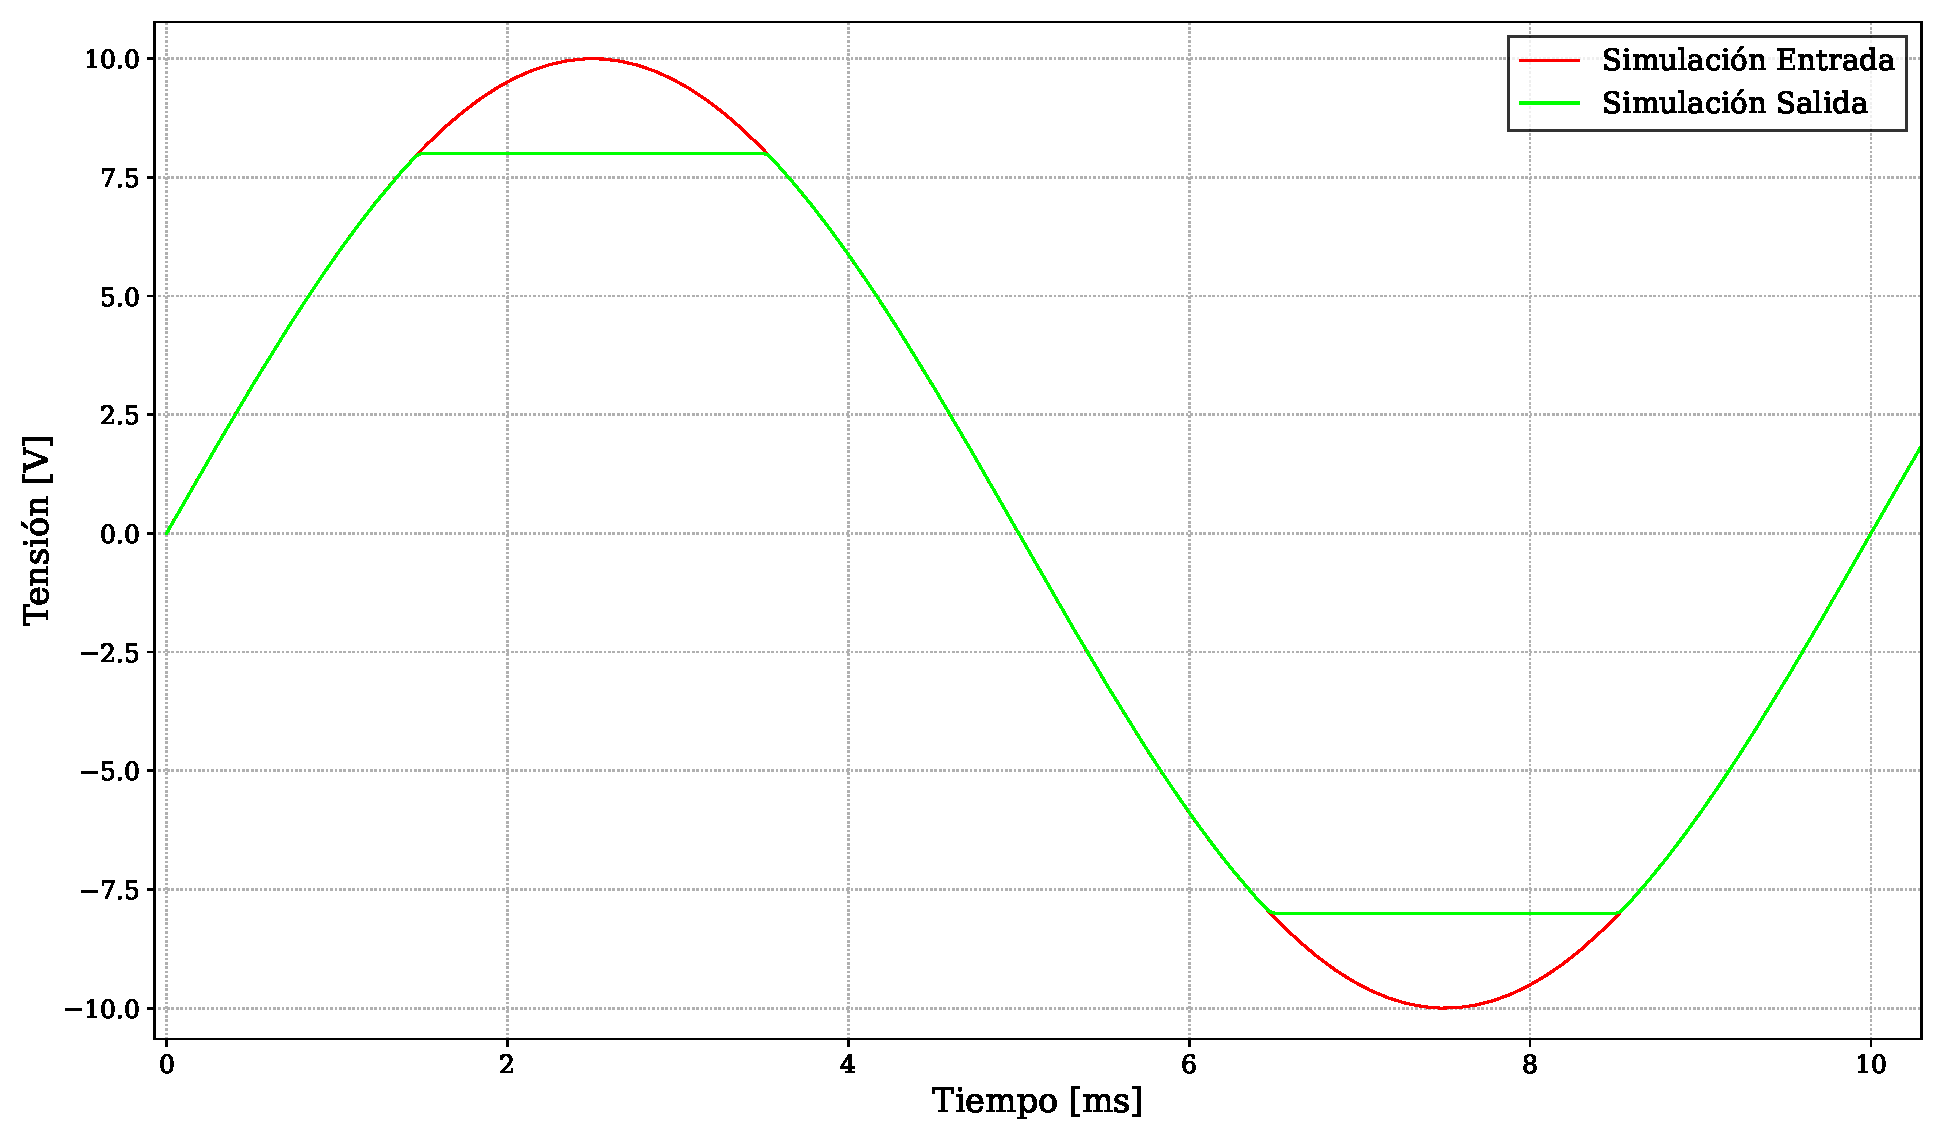
\includegraphics[width=\textwidth]{ej2f_teo.pdf} % Tu archivo PDF
    \caption{Curvas simuladas. Vin (rojo) y Vout (verde), la tensión que presenta clipping a la salida es de $\pm $8V.}
    \label{fig:pdf11}
  \end{minipage}
  \hfill % Espacio entre imágenes
  % Segunda imagen en PDF
  \begin{minipage}[b]{0.48\textwidth}
    \centering
    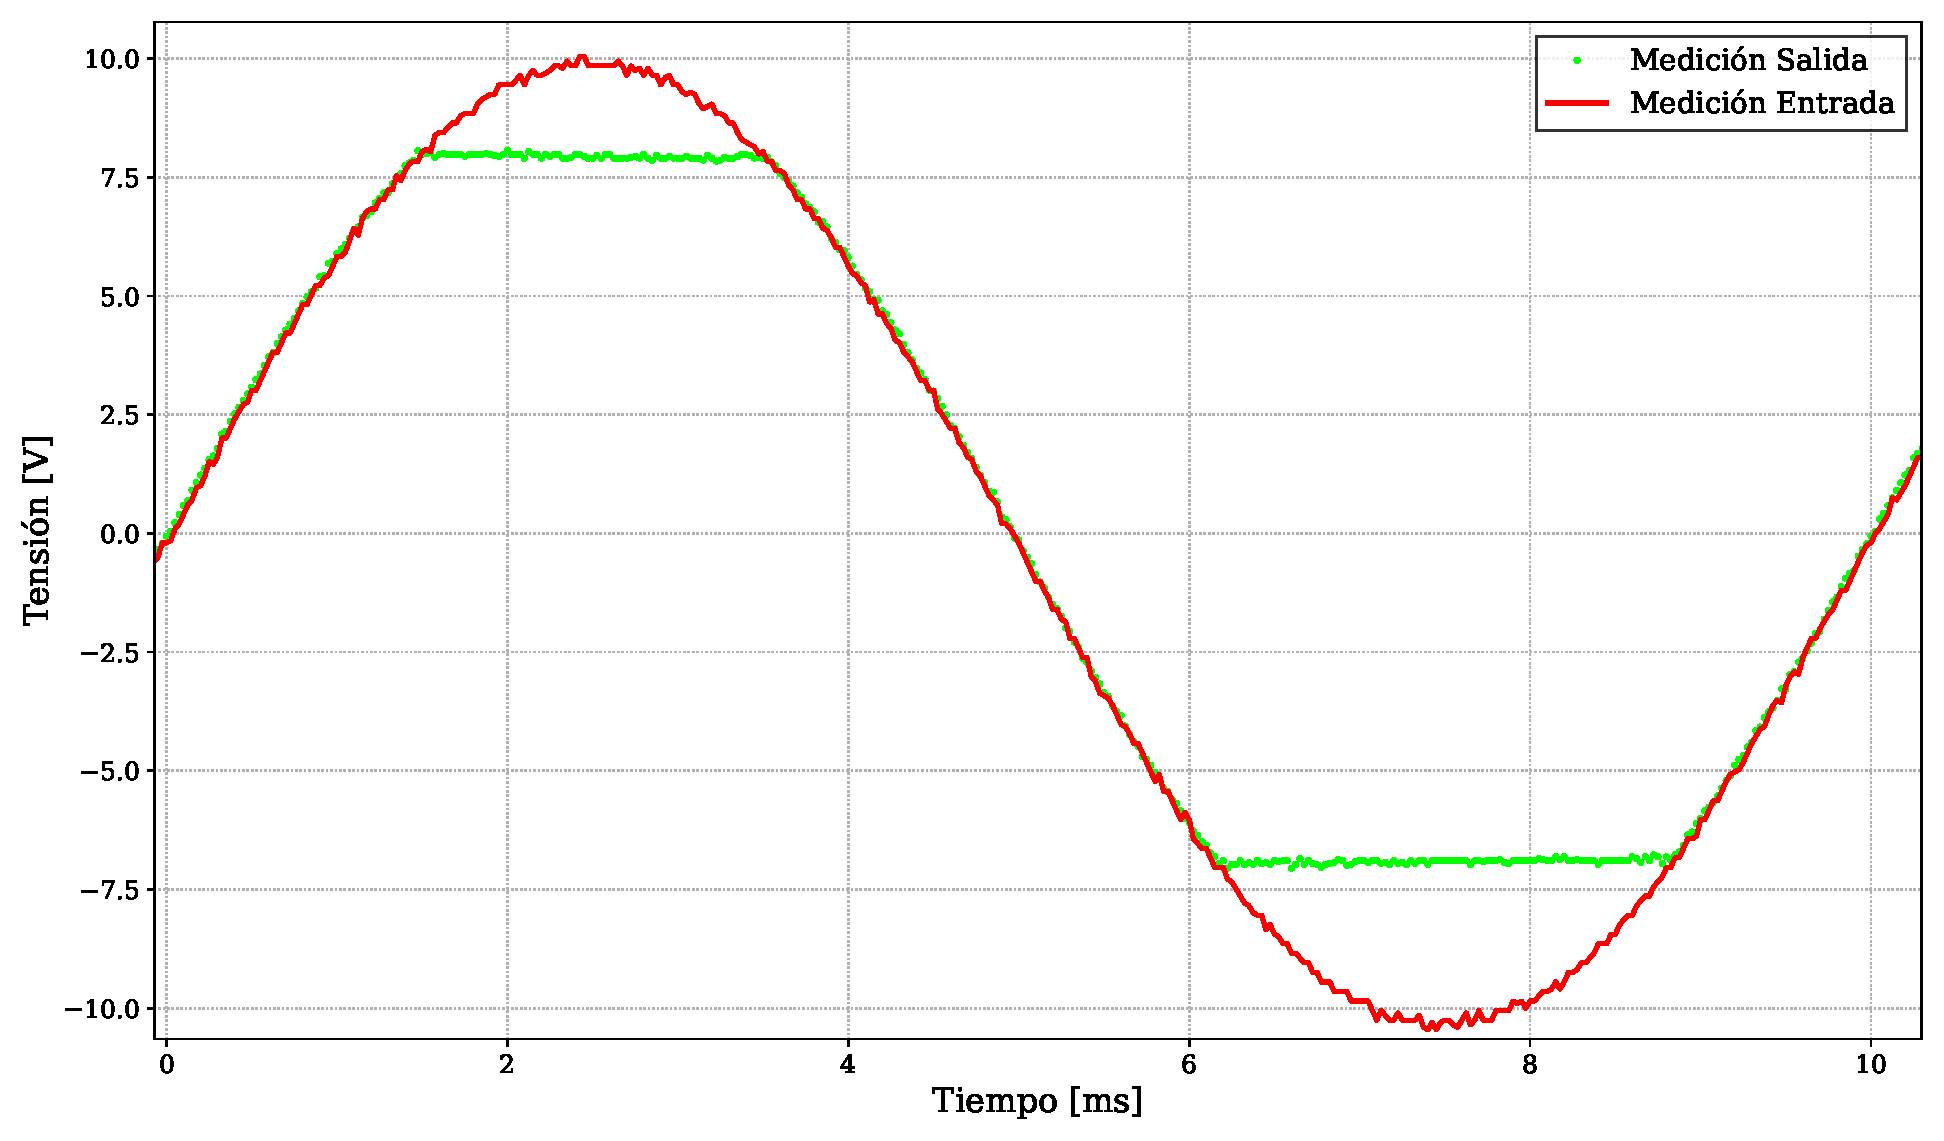
\includegraphics[width=\textwidth]{ej2f_prac.pdf} % Tu archivo PDF
    \caption{Curvas medidas. Vin (rojo) y Vout (verde), la tensión que presenta clipping a la salida en 7,9V y -7V.}
    \label{fig:pdf12}
  \end{minipage}
\end{figure}


\subsection{Caso G}

 \begin{table}[H]
\centering
\begin{tabular}{|c|c|c|c|c|c|c|c|}
\hline
Caso & $+V_{cc}\ [\text{V}]$ & $-V_{cc}\ [\text{V}]$ & $V_{DC}\ [\text{V}]$ &
 $V_p\ [\text{V}]$ & $f_{in}\ [\text{Hz}]$ & $R_L\ [\Omega]$ & Integrado \\ \hline
G & 10 & -10 & 0 & 8 & 800k & $\infty$ & TL072 \\ \hline
\end{tabular}
\end{table}

En este caso se puede ver algo particular, y es que no hay clipping por saturación 
como en el resto de casos, sino que la señal de salida no logra
''seguirle el paso'' a la señal de entrada. Esto se da por falta de ''slew rate'' del Op. Amp. que representa
la máxima pendiente en la entrada que es capaz de seguir sin deformarla. Una vez que se nota que la salida a)  
tiene cierto desfasaje con respecto a la entrada y b) tiene forma rectilínea cuando
 la entrada no lo es, tiene sentido pensar que el problema es la ''falta'' de slew rate del dispositivo.
 Ver las figuras \ref{fig:pdf13} y \ref{fig:pdf14}, observe que las pendientes 
 pronunciadas en la salida permiten incluso aproximar el Slew Rate (SR) del dispositivo con su pendiente. 
 Se buscó la pendiente cuando la salida aún está incrementando y resultó en un valor aproximado de 21$V/\mu s$, 
 y en el caso de la señal decrementando se obtuvo un valor de de módulo 15$V/\mu s$, y 
 comparándolo con el valor informado del SR en el datasheet (20$V/\mu s$), tienen sentido. Notar que
 el SR para señales de pendiente positiva es casi un tercio mayor que el SR para señales de pendiente negativa.
 Por otro lado, en el caso de la simulación, las pendientes en ambos casos coinciden, el valor de SR en la simulación es
 aproximadamente 13$V/\mu s$, otra prueba de que el modelo Spice de los componentes no es del todo confiable y se la debe considerar como una primera aproximación.

\begin{figure}[htbp]
  \centering
  % Primera imagen en PDF
  \begin{minipage}[b]{0.48\textwidth}
    \centering
    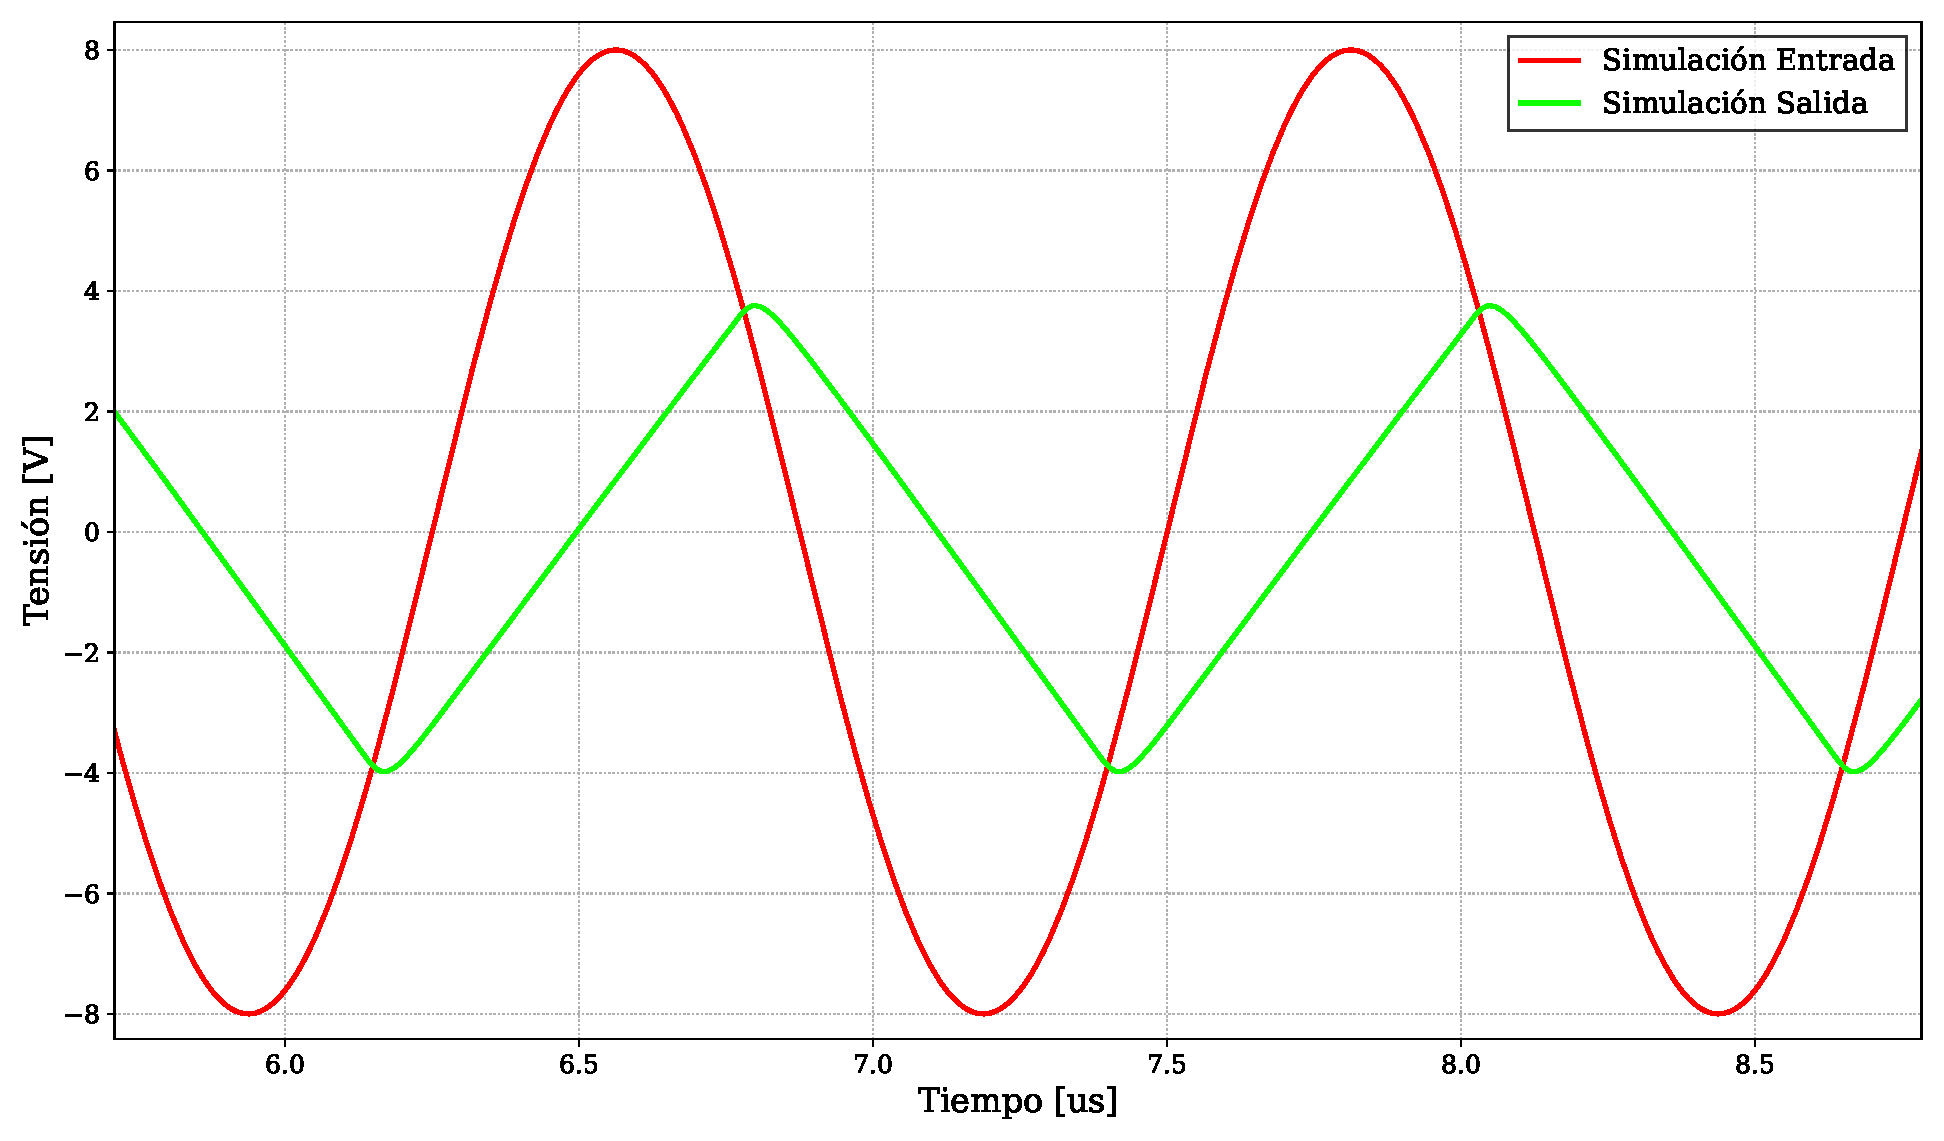
\includegraphics[width=\textwidth]{ej2g_teo.pdf} % Tu archivo PDF
    \caption{Curvas simuladas. Vin (rojo) y Vout (verde), las tensiones pico de la salida son 3,7V y -4V.}
    \label{fig:pdf13}
  \end{minipage}
  \hfill % Espacio entre imágenes
  % Segunda imagen en PDF
  \begin{minipage}[b]{0.48\textwidth}
    \centering
    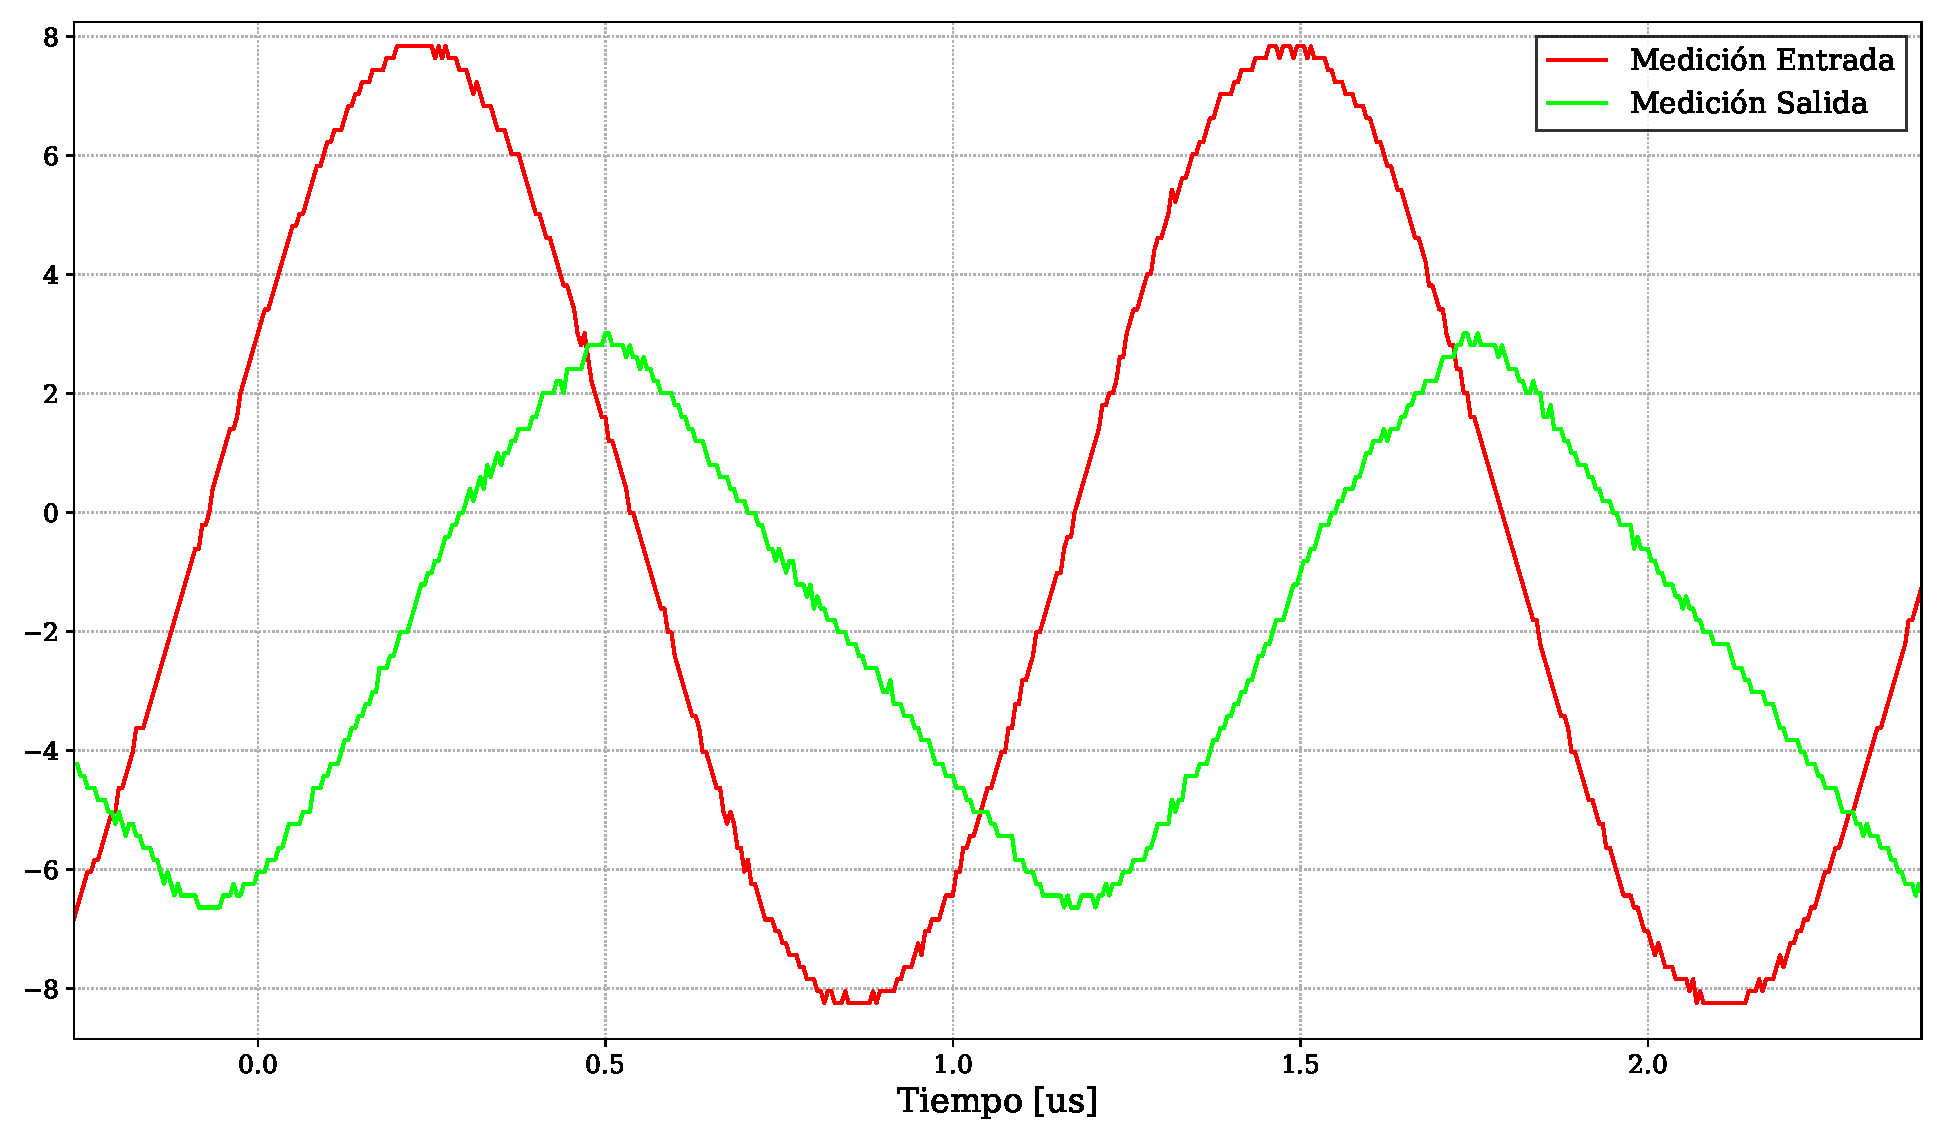
\includegraphics[width=\textwidth]{ej2g_prac.pdf} % Tu archivo PDF
    \caption{Curvas medidas. Vin (rojo) y Vout (verde), la tensiones pico de la salida son -6,6V y 2,9V.}
    \label{fig:pdf14}
  \end{minipage}
\end{figure}

\newpage
\section{Medición de la Ganancia de un Op. Amp.: TL082}

Uno pensaría que es posible medir la ganancia a lazo abierto o $A_{OL}$ a partir de un 
esquema como el de la figura \ref{fig:Ejc}. La única condición que queda a 
considerar es que la Vin sea lo suficientemente pequeña como para que multiplicada 
por $A_{OL}$, se obtenga un valor que se pueda medir a la salida del Op. Amp. 
Sin embargo, esto no funciona. Antes de justificarlo apropiadamente, es necesario introducir un nuevo concepto.
Los Op. Amp. fabricados presentan una distribución de posibles valores de un parámetro llamado $V_{offset}$.
 Así se lo denomina a la diferencia de potencial interna que se da entre el pin no inversor del exterior del 
 integrado y el nodo cuya tensión toma el dispositivo como la verdadera $V^{+}$ para luego amplificar. Es por esto
  que aún si se dejara en cortocircuito a las terminales inversora y no inversora, el operacional seguiría 
  “viendo” esa diferencia de tensión entre ellas. Por ejemplo, en la datasheet del TL082 (~\cite{datasheet_tl082}), se puede encontrar
   el valor aproximado de $V_{offset}$, que está en el orden de los mV. El problema de tener dicha diferencia de
    potencial, es que multiplicado por el $A_{OL}$, que suele ser del orden de $10^5$, la tensión que se debería
     obtener a la salida del Op. Amp. es del orden de los 100V, lo cual claramente deriva en una total saturación
      del dispositivo y por lo tanto en la falla al medir dicha tensión. Por eso, es que no importa 
      lo pequeña que sea la señal de Vin, con el circuito propuesto no es posible medir la ganancia a lazo abierto.
    \begin{figure}[htbp]
    \centering
    % Ajusta el ancho con respecto al texto (ej. 80% del ancho del texto)
    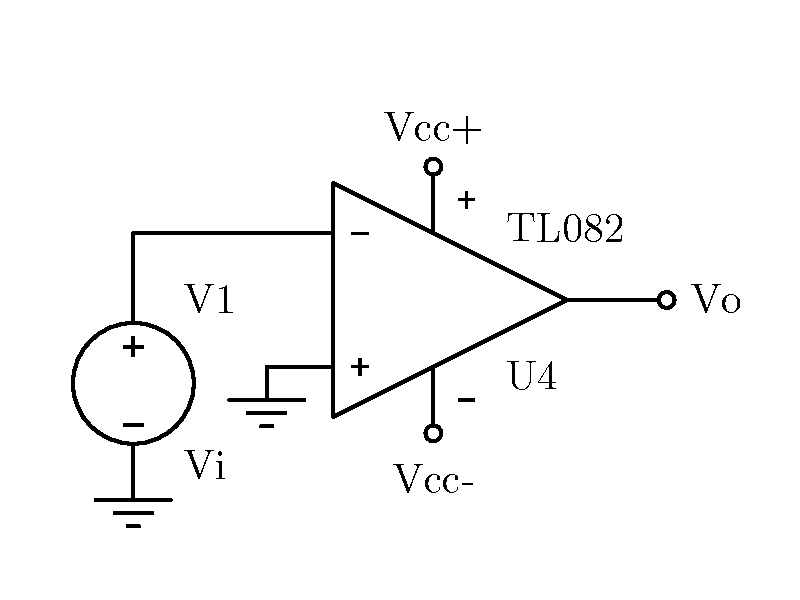
\includegraphics[width=0.4\textwidth]{Draft1.pdf} 
    \caption{Circuito propuesto para medición de $A_{OL}$.}
    \label{fig:Ejc}
\end{figure}


Ahora bien, a continuación se propone una manera de medir dicha ganancia 
utilizando los dos Op. Amp. del integrado TL082 con el circuito indicado en la 
figura \ref{fig:Ejc2}. 

Notese que partiendo de $Vout1=Vg+V_{offset2}$ (siendo $V_{offset2}$ la tensión de
 offset del Op. Amp. auxiliar), se puede deducir que la terminal no inversora interna, antes de pasar por la ''fuente de tensión'' de $V_offset$ ($V^{+}$) del DUT
está a una tensión de Vg dividido por $A_{OL}$ (se desprecia el valor de $\frac{V_offset2}{A_{OL}}$), y si se desprecia la corriente que le ingresa a las terminales del 
DUT se puede ver que entre Vout2 y $V^{+}-V_{offset}$, (ahora si, pasando por la fuente de tensión de $V_offset$) hay un divisor resistivo con las resistencias de $100k \Omega$ y $100 \Omega$.
Entonces, observe que $Vout2= (V^{+}-V_{offset})\cdot 1000=(\frac{Vg}{A_{OL}}-V_{Offset})\cdot 1000$.
 De esta forma, midiendo Vout2 se puede despejar el Offset con Vg=0V, que en la práctica resultó de 2,429mV,
 y luego con diferentes señales senoidales se pudo despejar el $A_{OL}$ del DUT, y en particular con una Vg continua.

En la figura \ref{fig:Ej3} se ve un ejemplo de una de las mediciones, en donde se colocó en Vg una senoidal de amplitud 15V (Vout1), frecuencia de 1kHz y se obtuvo una senoidal de amplitud 5 (Vout2).
Con dichos valores se despejó la ganancia del OA, que resultó valer 3000 en esa frecuencia.

En continua, se realizó la medición y se obtuvo como resultado un $A_{OL}=165268$, lo cual entra en el rango de lo esperable propuesto en la datasheet del dispositivo (valor típico de 200000).
En general, se realizaron mediciones que resultaron en los siguientes valores:
 10kHz, $A_{OL}=300$; 100Hz, $A_{OL}=28037$; 50Hz, $A_{OL}=53636$.
Sería esperable que cada par de valores resultara en el mismo GBWP, por lo que se lo calculó y se obtuvo, siguiendo el mismo orden de pares ya mencionados, comenzando por el
par de 10kHz: 3MHz; 2,8MHz; 2,7Mhz. De la misma forma, se considera que los resultados son los esperables según 
el valor informado en la datasheet(3MHz). Además, se puede calcular el valor de omega de corte,
 que indicaría la frecuencia en la que se encuentra el polo dominante con el que se fabrican los 
 Op. Amp. en general. A partir del valor de ganancia a lazo abierto obtenido en continua y utilizando
  la definición de GBWP y utilizando el valor de $BW \approx 3M$, se obtiene el valor 
  $f_{corte/polo\cdot dominante}=18Hz$, lo cual es esperable. 


\begin{figure}[htbp]
  \centering
  % Primera imagen en PD
    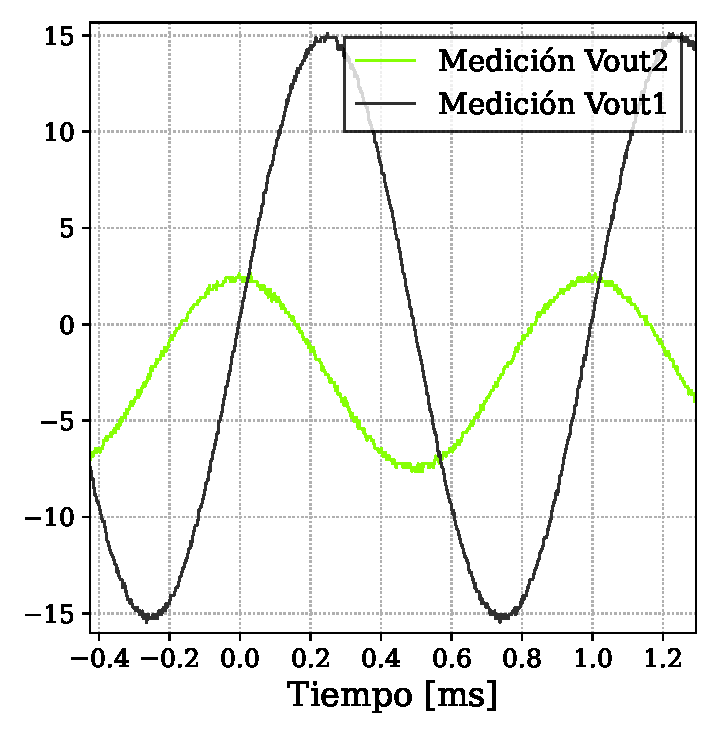
\includegraphics[width=0.6\textwidth]{ej3_prac.pdf} % Tu archivo PDF
    \caption{Medición Vout1-Vout2 para luego obtener valor de ganancia del DUT en la frecuencia de excitación (1kHz).}
    \label{fig:Ej3}
\end{figure}

\begin{figure}[htbp]
  \centering
  % Primera imagen en PD
    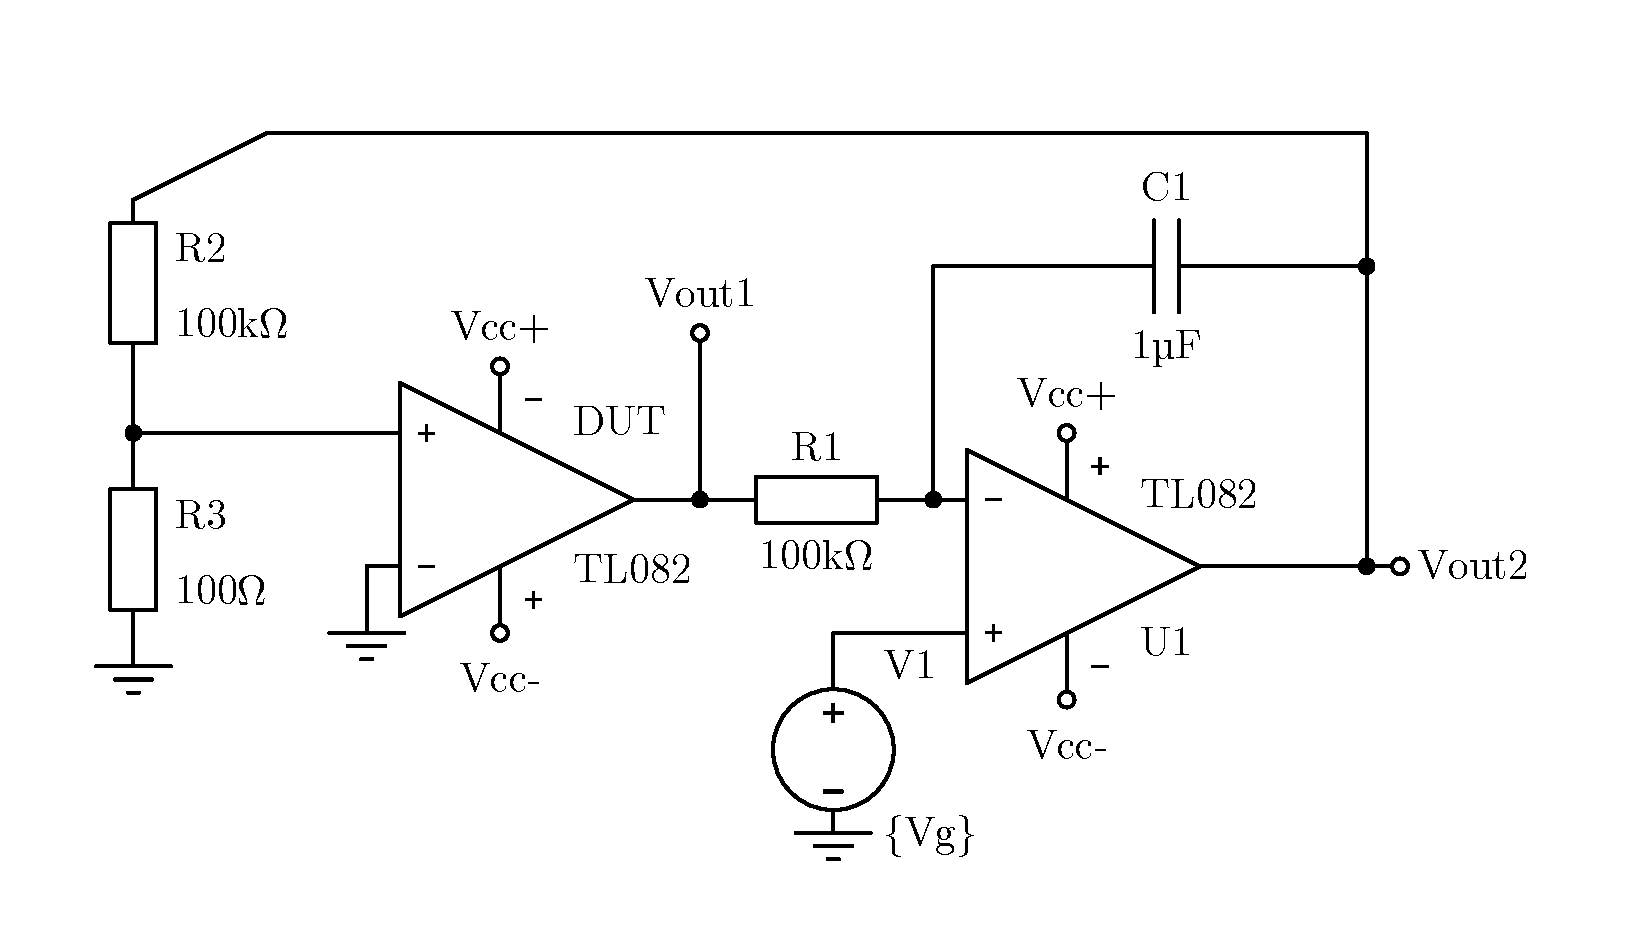
\includegraphics[width=0.6\textwidth]{Draft3.pdf} % Tu archivo PDF
    \caption{Circuito para medir $V_{offset}$ del Op. Amp. analizado (llamado DUT) si la fuente V1 se deja apagada. Si se la prende se podrá medir el $A_{OL}$ para diferentes frecuencias.}
    \label{fig:Ejc2}
\end{figure}

\section{Conclusión}
Finalmente, luego de trabajar con los dispositivos LM741, TL082 y TL072, se concluye que al no usar a los OA en la región de operación recomendada 
quedan al descubierto efectos no ideales como el Phase Reversal, la limitación de Slew Rate,
y la resistencia de salida $r_o$, incluso las limitaciones por saturación. Notese que 
dependiendo de la calidad del operacional utilizado, 
se puede ver como este tipo de factores se ve distorsionado, con respecto a lo informado por 
los fabricantes. Además, en la última sección se pudo comprobar que efectivamente los dispositivos se construyen con un polo dominante agregado para evitar problemas de inversión de fase al llegar hasta cierta frecuencia de señal de entrada.
Es interesante notar la utilidad que estos dispositivos ofrecen como en el caso de la búsqueda 
de la ganancia a lazo abierto de uno de ellos implementando un Servo Loop. 



\vspace{0cm}
\begin{thebibliography}{9}

\bibitem{datasheet_opamp}
  Texas Instruments,
  \textit{LM741 Operational Amplifier Datasheet},
  2015.
  [En línea]. Disponible en: \url{https://www.ti.com/lit/ds/symlink/lm741.pdf}

\bibitem{datasheet_tl072}
  Texas Instruments,
  \textit{TL07xx Low-Noise JFET-Input Operational Amplifiers Datasheet},
  Doc. SLOS080, 2021.
  [En línea]. Disponible en: \url{https://www.ti.com/lit/ds/symlink/tl072.pdf}

  \bibitem{analog_phase_reversal}
  W. Kester,
  \textit{Op Amp Input Overvoltage Protection and Phase Reversal},
  Analog Devices, Tutorial MT-036, 2009.
  [En línea]. Disponible en: \url{https://www.analog.com/media/en/training-seminars/tutorials/MT-036.pdf}

 \bibitem{datasheet_tl082}
  Texas Instruments,
  \textit{TL08xx General-Purpose JFET-Input Operational Amplifiers Datasheet},
  Doc. SLOS081, 2024.
  [En línea]. Disponible en: \url{https://www.ti.com/lit/ds/symlink/tl082.pdf}

\end{thebibliography}
\section{Anexo}

  

\begin{figure}[htbp]
    \centering
    % Ajusta el ancho con respecto al texto (ej. 80% del ancho del texto)
    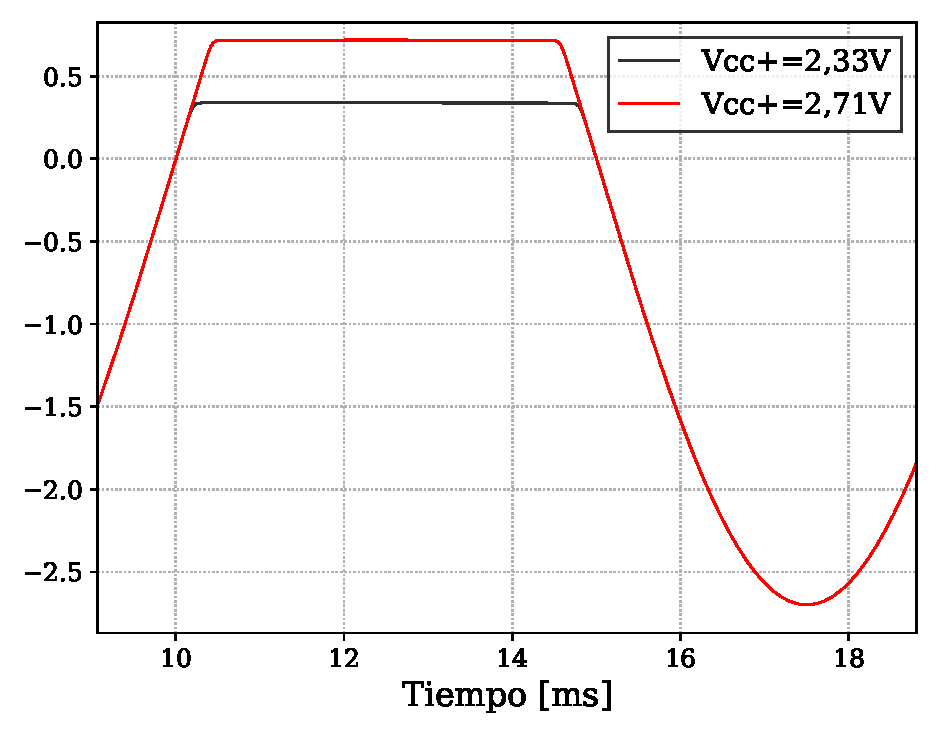
\includegraphics[width=0.6\textwidth]{anexo_lm741sittyvcc.pdf} 
    \caption{Salida del circuito del caso C con un LM741, con diferentes valores de Vcc+. Las tensiones de saturación son 0,71V y 0,33V para los casos de Vcc+ igual a 2,71V y 2,33V respectivamente, casualmente (Vcc+)-2V\dots}
    \label{fig:curiosidad2}
\end{figure}
%%% test%%
        
\end{document}
